\documentclass[11pt,a4paper]{report}
\usepackage[utf8]{inputenc}
\usepackage[english]{babel}
\usepackage[T1]{fontenc}
\usepackage{geometry}
\geometry{margin=1in}
\usepackage{hyperref}
\hypersetup{
    colorlinks=true,
    linkcolor=blue,
    filecolor=magenta,      
    urlcolor=cyan,
    pdftitle={GameHub Architecture Specification v3},
    pdfpagemode=FullScreen,
}
\usepackage{array}
\usepackage{booktabs}
\usepackage{longtable}
\usepackage{listings}
\usepackage{xcolor}
\usepackage{tikz}
\usetikzlibrary{shapes.geometric, arrows, positioning}
\usepackage{amsmath}
\usepackage{amssymb}
\usepackage{fancyhdr}
\usepackage{tcolorbox}
\usepackage{float}

% Listings styling
\definecolor{codegreen}{rgb}{0,0.6,0}
\definecolor{codegray}{rgb}{0.5,0.5,0.5}
\definecolor{codepurple}{rgb}{0.58,0,0.82}
\definecolor{backcolour}{rgb}{0.95,0.95,0.92}

\lstdefinestyle{mystyle}{
    backgroundcolor=\color{backcolour},   
    commentstyle=\color{codegreen},
    keywordstyle=\color{magenta},
    numberstyle=\tiny\color{codegray},
    stringstyle=\color{codepurple},
    basicstyle=\ttfamily\footnotesize,
    breakatwhitespace=false,         
    breaklines=true,                 
    captionpos=b,                    
    keepspaces=true,                 
    numbers=left,                    
    numbersep=5pt,                  
    showspaces=false,                
    showstringspaces=false,
    showtabs=false,                  
    tabsize=2
}
\lstset{style=mystyle}

\title{GameHub Architecture Specification v3\\ \large High-Scale Production System Blueprint}
\author{Principal Software Architect, Staff Engineer, DevOps Architect, Security Architect}
\date{\today}

\begin{document}

\maketitle
\tableofcontents
\newpage


\chapter{Executive Summary \& System Typologies}


\section{Introduction \& System Goals}
The GameHub system is transitioning from a Minimum Viable Product (MVP) to a high-scale production deployment. The system serves as a unified campus sports, matchmaking, and reservation portal. Key system constraints include strict consistency for ELO ledgers, low-latency matching, physical resource constraints (play area bookings), offline support for mobile PWA platforms, and high-concurrency event scoring.

\subsection{Physical Resource Sharing \& Limits (Admin-Configured)}
\begin{itemize}
    \item \textbf{Dynamic Physical PlayAreas}: The total count and distribution of physical assets (Pebolim, PingPong, Snooker, Bola 8, etc.) are dynamically managed by administrators rather than being hardcoded in application logic, schemas, or initial seeds. Administrators can dynamically create, assign, and alter physical table instances.
    \item \textbf{Multi-Game Shared Resource Mapping}: A single physical play area (e.g., a billiard table) can support multiple game types simultaneously (e.g., both \texttt{BOLA\_8} and \texttt{SNOOKER}).
    \item \textbf{Conflict Blocking Policy}: Reserving or booking a timeslot for a specific game type on a shared physical play area dynamically blocks all other supported game types on that specific play area for that exact time window to prevent overlapping reservation conflicts.
\end{itemize}

\subsection{Virtual Space Lifecycle}
\begin{itemize}
    \item \textbf{Card Games (TRUCO, BURACO)}: Card games require zero physical infrastructure. They support programmatic dynamic initialization and immediate automatic deletion upon match finalization. These transient virtual spaces completely bypass physical slot allocation validations, database checks, and optimistic concurrency control (OCC) constraints.
\end{itemize}


\section{Data Privacy Anonymization \& Identity Scrubbing Strategy}

To comply with global data protection regulations while preserving historical competitive data, the Game Hub defines a strict strategy boundary for user account deletions:
\begin{itemize}
    \item \textbf{Identity Scrubbing}: All sensitive personally identifiable information (PII) including \texttt{fullName}, \texttt{email}, and \texttt{nusp} is permanently wiped or replaced with randomized anonymized placeholders (e.g., \texttt{deleted\_user\_12345}).
    \item \textbf{Relational Integrity}: The historical records in the \texttt{EloLedger}, \texttt{MatchParticipant} score history, team roster logs, and administrative audit trails remain intact. Relational foreign keys pointing to the user's UUID are preserved to prevent data corruption and ensure seasons stats and ELO progression indices of other players are not altered.
\end{itemize}

\newpage

\section{Unified Business Capabilities Map}

The business design is driven by six core capabilities that represent the functional scope of the Game Hub:
\begin{enumerate}
    \item \textbf{Identity Management (RBAC)}: Governs registration, Course and Institute boundaries, User preferences, notification registration, and Role-Based Access Control (RBAC) claims.
    \item \textbf{Facility \& Equipment Coordination}: Coordinates physical recreation areas (PlayAreas), schedules reservations, controls hardware loans (Equipments, such as billiard cues and ping-pong paddles), and manages maintenance statuses.
    \item \textbf{Core Matchmaking \& Match Engine}: Manages active queuing systems, validates player ratings, tracks live heartbeats, records match scores, and coordinates set progressions.
    \item \textbf{Competition Slots \& Brackets}: Coordinates tournament match slots (and brackets) and calculates progression states for academic tournaments (elimination and round-robin).
    \item \textbf{ELO Engine Progression}: Evaluates match outcome details to execute rating adjustments at the close of active game sets, tracking ranking progression across competitive seasons.
    \item \textbf{Moderation \& Social Telemetry}: Governs friendships, peer communication channels, dispute reviews for contested match outcomes, and automatic user sanctions for negative behaviors.
\end{enumerate}

\newpage

\section{Modular Monolith Structural Design}
To maintain developer velocity, minimize operations overhead, and prevent premature microservices decomposition, GameHub is designed as a structured Modular Monolith using NestJS. 
The monolith is composed of independent, loosely coupled modules with strict boundaries. Communication between modules is mediated through well-defined module APIs, asynchronous in-memory event buses, or strict transaction-boundary contracts.

\subsection{Domain Boundaries}
The domain boundaries are aligned with Domain-Driven Design (DDD) principles:
\begin{enumerate}
    \item \textbf{Identity \& Teams Domain}: Manages users, roles, team rosters, and membership state.
    \item \textbf{Facilities Domain}: Governs courts, tables, play areas, and timeslot-based reservations.
    \item \textbf{Matchmaking Domain}: Handles active matching tickets, grouping algorithms, queue management, and pairing triggers.
    \item \textbf{Matches \& Progression Domain}: Manages match lifecycles, ELO updates via transactional ledger entries, and seasonal rankings.
    \item \textbf{Events \& Tournaments Domain}: Governs single/double elimination bracket structures, event configurations, and score summaries.
    \item \textbf{Social \& Moderation Domain}: Manages dispute resolutions, real-time match chats, report logs, and user access sanctions.
\end{enumerate}

\subsection{Module Boundary Enforcement Rules}
To prevent the codebase from degrading into a ``big ball of mud'', the following architectural constraints are enforced:
\begin{itemize}
    \item \textbf{Circular Dependencies}: Prohibited. Checked at build time via dependency-cruiser and linting rules.
    \item \textbf{Database Access}: Each module owns its schema tables. Cross-module database queries or joins are strictly forbidden. Access to data owned by another module must go through that module's exported service API.
    \item \textbf{Shared Kernels}: Limited to shared types, utility helpers, and common domain events.
\end{itemize}

\section{Hexagonal Architecture (Ports \& Adapters)}
Within each module, dependency inversion is maintained using Hexagonal Architecture. The core business logic is isolated from external frameworks, database drivers, and communication protocols.

\subsection{Structural Layers}
\begin{enumerate}
    \item \textbf{Domain Model (Core)}: Contains pure business logic, entities, value objects, and domain exceptions. No external dependencies.
    \item \textbf{Ports (Interfaces)}:
        \begin{itemize}
            \item \emph{Inbound Ports (Use Cases)}: Define commands, queries, and orchestration flows.
            \item \emph{Outbound Ports (Gateways)}: Define abstract interfaces for persistence, message queues, push notification services, and cache operations.
        \end{itemize}
    \item \textbf{Adapters (Infrastructure)}:
        \begin{itemize}
            \item \emph{Inbound Adapters (Primary)}: REST controllers, Socket.io gateways, background job consumers.
            \item \emph{Outbound Adapters (Secondary)}: PostgreSQL repositories via TypeORM, Redis caching operations, BullMQ job triggers.
        \end{itemize}
\end{enumerate}

\section{Core Data Flows}

\subsection{Matchmaking to Match Creation Flow}
\begin{enumerate}
    \item A \texttt{User} submits a \texttt{MatchmakingTicket}.
    \item The Matchmaking module places the ticket in a Redis-backed queue managed by BullMQ.
    \item A matchmaking worker aggregates tickets and groups users based on matching criteria (skill rating, location, latency).
    \item On pairing, a \texttt{Match} entity is initialized in a \texttt{PENDING} state.
    \item The Matchmaking module invokes the Facilities module to provision a \texttt{PlayAreaReservation} on a matching \texttt{PlayArea}.
    \item Once reservation is confirmed, the \texttt{Match} moves to \texttt{SCHEDULED} state.
    \item Players are notified via real-time WebSocket connection.
\end{enumerate}

\subsection{Match Finalization, Progression, and Score Flow}
\begin{enumerate}
    \item The match is completed. Match scores are submitted.
    \item The Match module marks the match as \texttt{COMPLETED}.
    \item The Match module publishes a \texttt{MatchFinalizedEvent}.
    \item \textbf{Progression Module Listener}:
        \begin{itemize}
            \item Appends ELO change vectors into the transactional \texttt{EloLedger}.
            \item Recalculates \texttt{PlayerRanking} scores.
        \end{itemize}
    \item \textbf{Events Module Listener}:
        \begin{itemize}
            \item Updates tournament bracket trees if the match is part of an active \texttt{Tournament}.
            \item Computes points and updates \texttt{EventScore} records.
        \end{itemize}
\end{enumerate}

\subsection{Dispute and Sanction Workflow}
\begin{enumerate}
    \item If users report incorrect results, a \texttt{MatchDispute} is created.
    \item Creating a dispute transitions the associated ELO updates in the ELO ledger to a \texttt{LOCKED} state.
    \item Moderation staff are notified via admin dashboards.
    \item If malicious behavior is confirmed, a \texttt{UserSanction} is placed against the offending user, blocking matchmaking access.
    \item Once resolved, ELO ledger records are unlocked and corrected.
\end{enumerate}

\section{State Machine \& Lifecycle Resilience}
Mobile systems frequently experience network drops and thread suspensions during backgrounding transitions. To prevent false-positive forfeits, the NestJS gateway processes the client-side \texttt{minimize\_presence} lifecycle event:
\begin{itemize}
    \item \textbf{Event Capture}: The mobile web client (wrapped via Capacitor) listens to the OS lifecycle changes. When backgrounding is detected, it broadcasts \texttt{minimize\_presence} to the WebSocket gateway.
    \item \textbf{Dynamic TTL Extension}: The gateway catches this event and extends the associated player's Redis heartbeat TTL key from the default 10 seconds to 60 seconds.
    \item \textbf{Worker Actions}: If the player resumes within 60 seconds, a standard heartbeat resets the TTL to 10 seconds. Otherwise, the status is flagged as disconnected, triggering the forfeit flow.
\end{itemize}

\section{Storage \& Concurrency Controls}
To avoid booking overlaps under high concurrency (e.g., peak tournament hours), the system implements the ``Matched but Homeless'' recovery strategy using Optimistic Concurrency Control (OCC) and transactional retries.

\subsection{TypeORM Mapping Template with Versioning}
The entity model for \texttt{PlayArea} employs an optimistic version control structure:
\begin{lstlisting}[caption={PlayArea Entity TypeORM Definition}]
import { Entity, PrimaryGeneratedColumn, Column, VersionColumn, OneToMany } from "typeorm";
import { PlayAreaReservation } from "./PlayAreaReservation.entity";

@Entity("play_areas")
export class PlayArea {
  @PrimaryGeneratedColumn("uuid")
  id: string;

  @Column({ type: "varchar", length: 100 })
  name: string;

  @Column({ type: "boolean", default: true })
  isActive: boolean;

  @VersionColumn()
  version: number;

  @OneToMany(() => PlayAreaReservation, (reservation) => reservation.playArea)
  reservations: PlayAreaReservation[];
}
\end{lstlisting}

\subsection{OCC Fallback \& Recovery Control Flow}
\begin{enumerate}
    \item A matchmaking match is paired and scheduled.
    \item In a transaction context, the allocation worker attempts to insert a \texttt{PlayAreaReservation} linking the \texttt{PlayArea} at timeslot $T$.
    \item The worker checks the version and updates the \texttt{PlayArea} using:
        \texttt{UPDATE play\_areas SET version = version + 1 WHERE id = :id AND version = :version}
    \item If the update count returns 0, the system throws an \texttt{OptimisticLockFailedException}.
    \item \textbf{Recovery Routine}: The match creation transaction rolls back immediately. The players' tickets are pushed back to the front of the active BullMQ queue using a high-priority job configuration, ensuring immediate rematching.
\end{enumerate}

\section{Security \& Authentication Architecture}
The system enforces a strict dual-token authentication model, incorporating native client storage fallback paths to handle WebKit Intelligent Tracking Prevention (ITP) restrictions on mobile iOS shells.

\subsection{Authentication Flow \& PIN Validation}
\begin{itemize}
    \item \textbf{4-Digit Numerical PIN Validation}: The system profile authentication utilizes a 4-digit numerical PIN (securely hashed, e.g., via Argon2) rather than a generic alphanumeric password string, facilitating rapid and secure entry on physical terminal kiosks and mobile shells.
    \item \textbf{Web Client Mode}: On successful login via valid 4-digit PIN verification, the server returns a short-lived access token in the JSON body, and sets a long-lived refresh token in an \texttt{HttpOnly}, \texttt{Secure}, \texttt{SameSite=Strict} cookie.
    \item \textbf{Mobile Shell (Capacitor) Mode}: WebKit ITP frequently purges or blocks third-party and local cookies on hybrid mobile wrappers. To mitigate this, the API auth routing detects the user agent header. If a mobile shell is identified, it bypasses the HTTP cookie setup and returns both the access and refresh tokens inside the encrypted JSON response body.
    \item \textbf{Native Secure Storage}: The Capacitor shell captures these tokens and saves them using the native \texttt{CapacitorSecureStorage} adapter, which writes directly to the iOS Keychain or Android KeyStore. Subsequent requests inject the refresh token inside the HTTP \texttt{Authorization} headers during session updates.
\end{itemize}

\section{Notification Decoupling}
The application core contains no dependency on external notification endpoints (FCM, APNs). It interacts solely via ports.

\subsection{INotificationServicePort Interface}
\begin{lstlisting}[caption={Push Notification Port}]
export interface INotificationServicePort {
  sendPushNotification(
    targetToken: string,
    title: string,
    body: string,
    metadata?: Record<string, string>
  ): Promise<boolean>;
}
\end{lstlisting}

\subsection{FCM Adapter Contract Payload}
\begin{lstlisting}[caption={FCM Adapter Contract Payload}]
{
  "message": {
    "token": "fcm_token_xyz123",
    "notification": {
      "title": "Match Scheduled",
      "body": "Your match is scheduled at Court 1 at 14:00"
    },
    "data": {
      "matchId": "m_832918",
      "type": "MATCH_SCHEDULED"
    }
  }
}
\end{lstlisting}

\subsection{APNs Adapter Contract Payload}
\begin{lstlisting}[caption={APNs Adapter Contract Payload}]
{
  "aps": {
    "alert": {
      "title": "Match Scheduled",
      "body": "Your match is scheduled at Court 1 at 14:00"
    },
    "badge": 1,
    "sound": "default"
  },
  "matchId": "m_832918",
  "type": "MATCH_SCHEDULED"
}
\end{lstlisting}


\section{Technical Stack Overview}


The technology stack is selected to prioritize robust horizontal scaling, absolute compile-time type safety, operational simplicity, and modern offline accessibility.

\subsection{Backend Runtime \& Application Layer}
\begin{itemize}
    \item \textbf{Runtime}: \textbf{Node.js LTS (v20)} + \textbf{TypeScript v5}. Provides structural typing, fast startup performance, and native asynchronous scheduling natively suited for non-blocking networking.
    \item \textbf{Application Framework}: \textbf{NestJS v10}. Utilizes structured module interfaces, robust dependency injection, architectural patterns, and direct compatibility with Express and Socket.io gateways.
\end{itemize}

\subsection{Database \& Persistence Strategies}
\begin{itemize}
    \item \textbf{Relational Database}: \textbf{PostgreSQL v16}. Enforces atomic state machine transitions, complex cross-module query integrity where needed (by abstraction layers), and strong structural indices. Handles the \texttt{EloLedger} operations safely under high transactional isolation levels.
    \item \textbf{Object-Relational Mapping (ORM)}: \textbf{TypeORM v0.3}. TypeORM supports decorator-driven data modeling, repository patterns, migrations, and direct integration with NestJS databases.
\end{itemize}

\subsection{Caching, Realtime, \& Queue Management}
\begin{itemize}
    \item \textbf{In-Memory Store \& Cache}: \textbf{Redis v7}. Used for session mapping, active matchmaking ticket indexes, lock primitives, and distributed pub/sub communication channels for scaling horizontal Socket.io servers.
    \item \textbf{Message Broker \& Job Queue}: \textbf{BullMQ v5}. Integrates with Redis to implement delayed execution jobs, persistent queue processing, backoff retry limits, and distributed scheduling for tournaments and matchmaking cycles.
    \item \textbf{Realtime Communication Gateway}: \textbf{Socket.io v4}. Selected for standard WebSocket connectivity, heartbeat checks, automatic network reconnection algorithms, and room isolation groupings (e.g., match chats, live scoring lobbies).
\end{itemize}

\subsection{Authentication \& Security Infrastructure}
\begin{itemize}
    \item \textbf{Token Implementation}: JWT stateless access tokens with short lifetimes (15 minutes). Signed with RSA-256 private keys.
    \item \textbf{Session Persistence}: Long-lived refresh tokens stored inside secure, client-inaccessible, \texttt{HttpOnly}, \texttt{Secure}, \texttt{SameSite=Strict} cookie headers, protecting credentials against Cross-Site Scripting (XSS) and Session Hijacking.
    \item \textbf{Access Control}: Role-Based Access Control (RBAC) integrated into NestJS application controllers using routing guards.
\end{itemize}

\subsection{Frontend Framework \& Application Packaging}
\begin{itemize}
    \item \textbf{Client Runtime}: \textbf{React v18} + \textbf{TypeScript}. Structured component composition and state synchronization using functional logic.
    \item \textbf{Build Tooling}: \textbf{Vite v5}. Optimized hot reloading, standard module splitting, and rapid build processes.
    \item \textbf{Global Client State}: \textbf{Zustand}. Lightweight store architecture with zero context-re-render issues.
    \item \textbf{Server Cache Sync}: \textbf{TanStack Query v5} (React Query). Governs backend HTTP query lifecycles, automated refetches, and state synchronization.
    \item \textbf{Native Mobile Adapter}: \textbf{CapacitorJS v5}. Bundles React web assets into native Android and iOS applications, exposing platform hooks (push channels, lifecycle synchronization adapters) directly to the web runtime.
\end{itemize}

\subsection{Infrastructure \& Deployments}
\begin{itemize}
    \item \textbf{Deployment Model}: Monolithic containers running inside AWS Elastic Container Service (ECS) on AWS Fargate.
    \item \textbf{CDN \& Edge WAF}: Cloudflare. Manages standard Static Page distribution, DDoS shielding, and SSL/TLS edge routing.
    \item \textbf{Database Management}: Amazon RDS PostgreSQL with Multi-AZ replications.
    \item \textbf{Caching Management}: Amazon ElastiCache Redis.
\end{itemize}


\chapter{Complete OOP Domain Layer (No Truncation)}


Below are the complete, translated, and detailed class architectures from the V1 baseline specification. All variables, types, and logic are fully abstract and tech-stack-agnostic.

\section{Domain 1: Identity, RBAC \& Teams}
Manages security identities, Courses, Institutes, user preference presets, and teams.

\begin{lstlisting}[caption={Identity and Teams Class Definitions}]
class User {
    id: UUID;
    nusp: String;
    nickname: String;
    email: String;
    fullName: String;
    birthDate: Date;
    pinHash: String; // Securely hashed 4-digit numerical PIN
    avatarUrl: String; // Optional avatar image URL
    instituteId: UUID;
    courseId: UUID;
    availabilityStatus: AvailabilityStatus; // AVAILABLE, MATCHED, OFFLINE
    isDeleted: Boolean;
}

class PublicUserDTO {
    id: UUID;
    nickname: String;
    instituteId: UUID;
    courseId: UUID;
}

class PrivateUserDTO {
    nusp: String;
    email: String;
    fullName: String;
    birthDate: Date;
}

class Institute {
    id: UUID;
    name: String;
    description: String;
}

class Course {
    id: UUID;
    name: String;
    description: String;
}

class Role {
    id: UUID;
    name: String;
    description: String;
}

class UserRole {
    userId: UUID;
    roleId: UUID;
}

class UserPreferences {
    userId: UUID;
    allowPushNotifs: Boolean;
    muteLobbyChat: Boolean;
    theme: String;
    soundEffectsEnabled: Boolean;
    vibrationEnabled: Boolean;
}

class DeviceToken {
    userId: UUID;
    tokenString: String;
    platform: String; // IOS, ANDROID
    lastUsedAt: DateTime;
}

abstract class Team {
    id: UUID;
    name: String;
    captainId: UUID;
    createdAt: DateTime;
}

class OfficialTeam extends Team {
    instituteId: UUID;
    isActiveCompetitionTeam: Boolean;
}

class TemporaryEventTeam extends Team {
    associatedEventId: UUID;
    expiresAt: DateTime;
}

class TeamRoster {
    teamId: UUID;
    userId: UUID;
    joinedAt: DateTime;
    status: RosterStatus; // ACTIVE, INVITATION_PENDING, REMOVED
    seedNumber: Integer;
}
\end{lstlisting}

\section{Domain 2: Facilities, Maintenance \& Equipment}
Coordinates physical resources, checkouts, and maintenance processes.

\begin{lstlisting}[caption={Facilities and Equipment Class Definitions}]
class PlayArea {
    id: UUID;
    name: String;
    supportedGameTypes: List<GameType>; // Admin-configured mapping (e.g., ['BOLA_8', 'SNOOKER'])
    status: PlayAreaStatus; // EMPTY, IN_USE, MAINTENANCE
    isVirtual: Boolean; // True for transient, dynamically spawned card game spaces (TRUCO, BURACO)
}

class PlayAreaReservation {
    id: UUID;
    playAreaId: UUID;
    userId: UUID;
    scheduledStartTime: DateTime;
    scheduledEndTime: DateTime;
    bufferPaddingMinutes: Integer; // In minutes, to absorb scheduling shifts
    status: ReservationStatus; // CONFIRMED, ACTIVE, COMPLETED, CANCELLED
    version: Integer;
}

class Equipment {
    id: UUID;
    name: String;
    serialNumber: String;
    type: String; // CUE, PADDLE, BALL_SET, CARD_DECK
    status: EquipmentStatus; // AVAILABLE, IN_USE, MAINTENANCE
    description: String;
}

class CheckoutRecord {
    id: UUID;
    equipmentId: UUID;
    userId: UUID;
    playAreaReservationId: UUID; // Optional, null if checked out without reservation association
    checkedOutAt: DateTime;
    returnedAt: DateTime;
    status: CheckoutStatus; // ACTIVE, RETURNED, OVERDUE
    returnCondition: ReturnCondition; // PRISTINE, WORN, DAMAGED
    associatedMaintenanceTicketId: UUID;
}

class MaintenanceTicket {
    id: UUID;
    resourceType: String; // PLAY_AREA, EQUIPMENT
    resourceId: UUID;
    reportedById: UUID;
    description: String;
    reportedAt: DateTime;
    resolvedAt: DateTime;
    status: MaintenanceStatus; // OPEN, INVESTIGATING, RESOLVED
}
\end{lstlisting}

\section{Domain 3: Matchmaking, Concurrency \& Core Engine}
This module contains the matching engine, live gameplay tracking, and physical allocation bounds.

\subsection{Forfeit Score Semantics}
To prevent structural null violations and numerical division-by-zero errors in ELO calculations, the domain models enforce a fallback scoring policy for abrupt match dropouts (e.g., when a heartbeat timeout triggers). The winning participant is credited with a default maximum score (such as $11$ or $2$), whereas the forfeiting side is locked at $0$.

\begin{lstlisting}[caption={Matchmaking and Core Gameplay Class Definitions}]
abstract class Game {
    id: UUID;
    name: String;
    gameType: GameType;
    minPlayers: Integer;
    maxPlayers: Integer;
    equipmentRequirements: List<EquipmentType>;
}

class TableGame extends Game {
    validatePhysicalBounds(): Boolean {
        // Dynamically tallies operational PlayArea records matching this game type
        // whose statuses are not flagged as MAINTENANCE to verify capacity bounds.
        return true;
    }
}

class CardGame extends Game {
    deckCount: Integer;
    requiresDealer: Boolean;
}

class MatchmakingTicket {
    id: UUID;
    userId: UUID;
    teamId: UUID; // Optional, null if individual matchmaking
    eloRating: Integer;
    gameType: GameType;
    joinedAt: DateTime;
    expiryTime: DateTime;
    status: TicketStatus; // WAITING, MATCHED, CANCELLED, EXPIRED
}

class Matchmaker {
    // Singleton controller logic to match waiting tickets within ELO ranges
    activeTickets: List<MatchmakingTicket>;
    
    matchmake(): List<Match> {
        // Core matchmaking algorithm: groups compatible tickets
        // Calculates ticket age (currentTime - MatchmakingTicket.joinedAt)
        // and scales open ELO range dynamically to minimize queues.
        // Defensively verifies (currentTime < ticket.expiryTime) before pairing.
        return new List<Match>();
    }
}

class Match {
    id: UUID;
    playAreaReservationId: UUID; // Optional, null for virtual card games
    gameType: GameType;
    status: MatchStatus; // PENDING_RESOURCE_ALLOCATION, IN_PROGRESS, COMPLETED, DISPUTED, CANCELLED
    startedAt: DateTime;
    endedAt: DateTime;
}

class MatchParticipant {
    matchId: UUID;
    userId: UUID;
    teamId: UUID; // Optional, null if individual match
    score: Integer;
    resultStatus: ParticipantResult; // WINNER, LOSER, FORFEITED, DISQUALIFIED
}

class MatchSet {
    id: UUID;
    matchId: UUID;
    setNumber: Integer;
    scoreSide1: Integer;
    scoreSide2: Integer;
    winnerId: UUID;
}

class MatchEvent {
    id: UUID;
    matchId: UUID;
    userId: UUID; // Instigator of the event
    eventType: String; // Ex: BALL_POTTED, FOUL, GAME_START
    details: String;
    timestamp: DateTime;
}
\end{lstlisting}

\section{Domain 4: Custom Events, Parties \& Tournaments}
Manages campus competitions, elimination stages, and match scoreboards.

\begin{lstlisting}[caption={Events and Tournaments Class Definitions}]
class Event {
    id: UUID;
    name: String;
    creatorId: UUID;
    description: String;
    startTime: DateTime;
    endTime: DateTime;
    status: EventStatus; // PLANNING, ACTIVE, COMPLETED
}

class EventScore {
    eventId: UUID;
    userId: UUID;
    scoreValue: Integer;
    lastUpdatedAt: DateTime;
}

class Tournament {
    id: UUID;
    name: String;
    gameId: UUID;
    format: TournamentFormat; // SINGLE_ELIMINATION, DOUBLE_ELIMINATION, ROUND_ROBIN
    registrationStartTime: DateTime;
    registrationEndTime: DateTime;
    status: TournamentStatus; // REGISTRATION, ACTIVE, CONCLUDED
}

class TournamentMatchSlot {
    id: UUID;
    tournamentId: UUID;
    roundNumber: Integer;
    matchId: UUID;
    parentSlotId: UUID; // Null for final round or Round-Robin stage
}

class GroupStanding {
    tournamentId: UUID;
    teamId: UUID;
    points: Integer;
    matchesWon: Integer;
    matchesLost: Integer;
    scoreDifferential: Integer;
}
\end{lstlisting}

\section{Domain 5: Academics \& Progression / ELO Engine}
Manages seasons, practice tracking, player rankings, and immutable ELO records.

\begin{lstlisting}[caption={Progression and ELO Class Definitions}]
class Season {
    id: UUID;
    name: String;
    startTime: DateTime;
    endTime: DateTime;
    isActive: Boolean;
}

class PracticeSession {
    id: UUID;
    playAreaId: UUID;
    startedAt: DateTime;
    endedAt: DateTime;
}

class PracticeAttendance {
    practiceSessionId: UUID;
    userId: UUID;
    checkInTime: DateTime;
}

class PlayerRanking {
    id: UUID;
    seasonId: UUID;
    userId: UUID;
    teamId: UUID; // Optional, null if individual ladder profile
    gameType: GameType;
    eloValue: Integer;
    gamesPlayed: Integer;
    lastMatchAt: DateTime;
}

class EloLedger {
    id: UUID;
    userId: UUID;
    teamId: UUID; // Optional, null if individual ladder transaction
    matchId: UUID;
    seasonId: UUID;
    oldRating: Integer;
    newRating: Integer;
    changeAmount: Integer;
    calculatedAt: DateTime;
}
\end{lstlisting}

\section{Domain 6: Social, Moderation \& Telemetry}
Governs relationships, chats, reports, security bans, and performance monitoring.

\begin{lstlisting}[caption={Social and Telemetry Class Definitions}]
class Friendship {
    userId1: UUID;
    userId2: UUID;
    establishedAt: DateTime;
    status: FriendshipStatus; // PENDING, ACCEPTED, BLOCKED
}

class ChatChannel {
    id: UUID;
    type: ChannelType; // PRIVATE_MESSAGE, LOBBY, MATCH_ROOM
    associatedResourceId: UUID; // Null if PM, matchId if MATCH_ROOM
}

class ChatMessage {
    id: UUID;
    channelId: UUID;
    senderId: UUID;
    content: String;
    sentAt: DateTime;
}

class MatchDispute {
    id: UUID;
    matchId: UUID;
    raisedById: UUID;
    reason: String;
    status: DisputeStatus; // UNDER_REVIEW, RESOLVED, DISMISSED
    resolvedAt: DateTime;
    resolvedById: UUID;
    resolutionNotes: String;
}

class GenericReport {
    id: UUID;
    reportedByUserId: UUID;
    targetUserId: UUID;
    reason: String;
    details: String;
    reportedAt: DateTime;
    status: ReportStatus; // OPEN, INVESTIGATING, CLOSED
}

class UserSanction {
    id: UUID;
    userId: UUID;
    type: SanctionType; // WARNING, TEMP_BAN, PERMANENT_BAN
    reason: String;
    startedAt: DateTime;
    expiresAt: DateTime;
    isActive: Boolean;
    createdById: UUID;
}

class SystemTelemetry {
    id: UUID;
    metricName: String; // Ex: MatchmakingQueueSize, APIResponseTime
    metricValue: Double;
    recordedAt: DateTime;
}
\end{lstlisting}

\section{Utility \& Core Debugging Utilities}
Aids system troubleshooting and game lifecycle simulations.

\begin{lstlisting}[caption={System Debugger Class Definitions}]
class StateDebugger {
    public dumpSystemState(): Map<String, Any> {
        // Collects in-memory queues and active reservations for audit
        return new Map<String, Any>();
    }
}

class MatchSimulatorLogger {
    public logSimulationEvent(matchId: UUID, logMessage: String): void {
        // Records dry-run matchmaking flows to debug calculations
    }
}
\end{lstlisting}


\chapter{Operational JSON \& Field Mappings}

\section{JSON Showcase: 8-Ball Pool (Bola 8) Scenario}
To validate the conceptual domain model against real-world operations, the following JSON snippet exemplifies a complete \textbf{8-Ball Pool (Bola 8)} match scenario.

\begin{lstlisting}[caption={Bola 8 Conceptual JSON Instance}]
{
  "User": {
    "id": "a1b2c3d4-e5f6-7a8b-9c0d-1e2f3a4b5c6d",
    "nusp": "12345678",
    "nickname": "PoolKing88",
    "email": "poolking@usp.br",
    "fullName": "Joao Silva",
    "birthDate": "2002-05-15",
    "instituteId": "b2c3d4e5-f6a7-8b9c-0d1e-2f3a4b5c6d7e",
    "courseId": "c3d4e5f6-a7b8-9c0d-1e2f-3a4b5c6d7e8f",
    "availabilityStatus": "MATCHED",
    "isDeleted": false
  },
  "PublicUserDTO": {
    "id": "a1b2c3d4-e5f6-7a8b-9c0d-1e2f3a4b5c6d",
    "nickname": "PoolKing88",
    "instituteId": "b2c3d4e5-f6a7-8b9c-0d1e-2f3a4b5c6d7e",
    "courseId": "c3d4e5f6-a7b8-9c0d-1e2f-3a4b5c6d7e8f"
  },
  "PrivateUserDTO": {
    "nusp": "12345678",
    "email": "poolking@usp.br",
    "fullName": "Joao Silva",
    "birthDate": "2002-05-15"
  },
  "TableGame": {
    "id": "d4e5f6a7-b8c9-0d1e-2f3a-4b5c6d7e8f9a",
    "name": "8-Ball Pool",
    "gameType": "BOLA_8",
    "minPlayers": 2,
    "maxPlayers": 2,
    "equipmentRequirements": ["CUE", "BALL_SET"]
  },
  "PlayArea": {
    "id": "e5f6a7b8-c9d0-1e2f-3a4b-5c6d7e8f9a0b",
    "name": "Billiard Table 01",
    "gameType": "BOLA_8",
    "status": "IN_USE",
    "version": 7
  },
  "PlayAreaReservation": {
    "id": "f6a7b8c9-d0e1-2f3a-4b5c-6d7e8f9a0b1c",
    "playAreaId": "e5f6a7b8-c9d0-1e2f-3a4b-5c6d7e8f9a0b",
    "userId": "a1b2c3d4-e5f6-7a8b-9c0d-1e2f3a4b5c6d",
    "scheduledStartTime": "2026-06-20T18:00:00Z",
    "scheduledEndTime": "2026-06-20T19:00:00Z",
    "bufferPaddingMinutes": 15,
    "status": "ACTIVE",
    "version": 2
  },
  "Equipment": {
    "id": "a7b8c9d0-e1f2-3a4b-5c6d-7e8f9a0b1c2d",
    "name": "Custom Ash 3/4 Billiard Cue",
    "serialNumber": "SN-CUE-ASH-9981",
    "type": "CUE",
    "status": "IN_USE",
    "description": "High-grade imported Ash wood cue with customized joint"
  },
  "CheckoutRecord": {
    "id": "b8c9d0e1-f2a3-4b5c-6d7e-8f9a0b1c2d3e",
    "equipmentId": "a7b8c9d0-e1f2-3a4b-5c6d-7e8f9a0b1c2d",
    "userId": "a1b2c3d4-e5f6-7a8b-9c0d-1e2f3a4b5c6d",
    "playAreaReservationId": "f6a7b8c9-d0e1-2f3a-4b5c-6d7e8f9a0b1c",
    "checkedOutAt": "2026-06-20T17:58:00Z",
    "returnedAt": null,
    "status": "ACTIVE",
    "returnCondition": null,
    "associatedMaintenanceTicketId": null
  },
  "MatchmakingTicket": {
    "id": "c9d0e1f2-a3b4-5c6d-7e8f-9a0b1c2d3e4f",
    "userId": "a1b2c3d4-e5f6-7a8b-9c0d-1e2f3a4b5c6d",
    "teamId": null,
    "eloRating": 1500,
    "gameType": "BOLA_8",
    "joinedAt": "2026-06-20T17:45:00Z",
    "expiryTime": "2026-06-20T17:55:00Z",
    "status": "MATCHED"
  },
  "Match": {
    "id": "d0e1f2a3-b4c5-6d7e-8f9a-0b1c2d3e4f5a",
    "playAreaReservationId": "f6a7b8c9-d0e1-2f3a-4b5c-6d7e8f9a0b1c",
    "gameType": "BOLA_8",
    "status": "IN_PROGRESS",
    "startedAt": "2026-06-20T18:02:00Z",
    "endedAt": null
  },
  "TeamRoster": {
    "teamId": "d0e1f2a3-b4c5-6d7e-8f9a-0b1c2d3e4f5b",
    "userId": "a1b2c3d4-e5f6-7a8b-9c0d-1e2f3a4b5c6d",
    "joinedAt": "2026-06-20T17:00:00Z",
    "status": "ACTIVE",
    "seedNumber": 1
  }
}
\end{lstlisting}

\section{Completeness Verification Matrix}

Table~\ref{tab:verification_matrix} registers all system domain classes, detailing their main purposes, core functions, expected lifecycles, and verification check status.

\begingroup
\setlength{\tabcolsep}{4pt}
\begin{longtable}{>{\raggedright\arraybackslash}p{2.8cm}>{\raggedright\arraybackslash}p{3.2cm}>{\raggedright\arraybackslash}p{3.2cm}>{\raggedright\arraybackslash}p{3.3cm}>{\raggedright\arraybackslash}p{2.0cm}}
\caption{Completeness Verification Matrix} \label{tab:verification_matrix} \\
\toprule
\textbf{Class Name} & \textbf{Abstract Purpose} & \textbf{Key Methods} & \textbf{Lifecycle States} & \textbf{Validation} \\
\midrule
\endfirsthead
\multicolumn{5}{c}%
{{\bfseries Table \thetable\ (continued from previous page)}} \\
\midrule
\textbf{Class Name} & \textbf{Abstract Purpose} & \textbf{Key Methods} & \textbf{Lifecycle States} & \textbf{Validation} \\
\midrule
\endhead
\bottomrule
\endfoot
\bottomrule
\endlastfoot

\texttt{User} & Security identity profile & \texttt{updateStatus()} & AVAILABLE, MATCHED, OFFLINE & Verified \\
\texttt{PlayArea} & Coordinates game tables & \texttt{validatePhysicalBounds()} & EMPTY, IN\_USE, MAINTENANCE & Verified \\
\texttt{PlayAreaReservation} & Manages slot bookings with padding & \texttt{confirmReservation()} & CONFIRMED, ACTIVE, CANCELLED & Verified \\
\texttt{Equipment} & Handles physical checkouts & \texttt{updateStatus()} & AVAILABLE, IN\_USE, MAINTENANCE & Verified \\
\texttt{CheckoutRecord} & Controls cue loans linked to reservation & \texttt{flagOverdue()} & ACTIVE, RETURNED, OVERDUE & Verified \\
\texttt{MatchmakingTicket} & Active queue ticket & \texttt{isExpired()} & WAITING, MATCHED, EXPIRED & Verified \\
\texttt{Match} & Regulates side-agnostic progressions & \texttt{processSetOutcome()} & PENDING\_RESOURCE\_ALLOCATION, IN\_PROGRESS, COMPLETED & Verified \\
\texttt{TournamentMatchSlot} & Structures tournament slots & \texttt{advanceWinner()} & PENDING, READY, COMPLETED & Verified \\
\texttt{EloLedger} & Tracks ranking changes & \texttt{recordEloChange()} & COMPLETED & Verified \\
\texttt{GroupStanding} & Handles group-stage standings & \texttt{calculateStanding()} & ACTIVE, CONCLUDED & Verified \\
\texttt{PublicUserDTO} & Filters non-sensitive user data & \texttt{serialize()} & ACTIVE & Verified \\
\texttt{PrivateUserDTO} & Holds sensitive RBAC user data & \texttt{serialize()} & ACTIVE & Verified \\
\end{longtable}
\endgroup


\chapter{Production Stack Adapter Specifications}

This chapter details the production-grade technology implementation of external adapter layers. All components implement the abstract ports defined in Chapter 2, separating core business logic from framework concerns.

\section{Core Runtime \& Backend Framework}

\subsection{Runtime \& Language: TypeScript on Node.js / Bun}

The application backend executes \textbf{TypeScript} compiled to a native runtime on either \textbf{Node.js} (LTS) or \textbf{Bun} (for environments prioritizing cold-start performance and minimal memory footprint). The central rationale is compile-time type fidelity: the abstract domain interfaces defined throughout the OOP class hierarchy (e.g., \texttt{IEnrollPlayerUseCase}, \texttt{IPlayAreaRepositoryPort}, \texttt{INotificationServicePort}) are expressed as TypeScript \texttt{interface} or \texttt{abstract class} constructs. This means the runtime carries zero ambiguity at the boundary between core domain logic and its concrete adapters.

\begin{lstlisting}[language=Java, caption={TypeScript abstract port interface mapping}]
// Output Port (abstract, lives inside Core Domain)
interface IPlayAreaRepositoryPort {
  findById(id: string): Promise<PlayArea | null>;
  updateWithOptimisticLock(
    area: PlayArea,
    expectedVersion: number
  ): Promise<void>;
}

// Concrete Adapter (lives in Infrastructure layer)
class TypeOrmPlayAreaAdapter implements IPlayAreaRepositoryPort {
  async findById(id: string): Promise<PlayArea | null> { ... }
  async updateWithOptimisticLock(
    area: PlayArea,
    expectedVersion: number
  ): Promise<void> { ... }
}
\end{lstlisting}

Because TypeScript enforces structural typing at compile time, attempting to pass a concrete adapter that does not satisfy the port contract becomes a build error, not a runtime exception. This gives the Hexagonal boundary a hard enforcement mechanism that a purely runtime language cannot replicate without extensive reflection overhead.

\subsection{Application Framework: NestJS with Strict Modular Architecture}

\textbf{NestJS} is selected as the application framework. Its module system maps directly to the six business domain capabilities defined in Section 2, producing one NestJS \texttt{Module} per domain: \texttt{IdentityModule}, \texttt{FacilitiesModule}, \texttt{MatchmakingModule}, \texttt{TournamentsModule}, \texttt{ProgressionModule}, and \texttt{SocialModule}.

The critical architectural guarantee is that NestJS's dependency injection (DI) container enforces the Hexagonal separation by using \textbf{custom injection tokens} rather than concrete class references in controller constructors. This prevents framework-layer controllers from importing or instantiating domain use cases directly.

\begin{lstlisting}[language=Java, caption={NestJS Hexagonal DI Token Pattern}]
// tokens.ts (shared constants, imported by module providers)
export const ENROLL_PLAYER_USE_CASE
  = Symbol('IEnrollPlayerUseCase');

// matchmaking.module.ts (Infrastructure/Framework layer)
@Module({
  providers: [
    {
      provide: ENROLL_PLAYER_USE_CASE,
      useClass: EnrollPlayerUseCase, // concrete application service
    },
    TypeOrmMatchmakingTicketAdapter,
    RedisMatchmakingQueueAdapter,
  ],
  controllers: [MatchmakingHttpController],
})
export class MatchmakingModule {}

// matchmaking-http.controller.ts
@Controller('/matchmaking')
export class MatchmakingHttpController {
  constructor(
    @Inject(ENROLL_PLAYER_USE_CASE)
    private readonly enrollPlayer: IEnrollPlayerUseCase,
  ) {}

  @Post('/queue')
  async joinQueue(@Body() dto: EnrollPlayerDto) {
    return this.enrollPlayer.execute(dto);
  }
}
\end{lstlisting}

The HTTP controller imports only the \texttt{IEnrollPlayerUseCase} interface type and the symbol token. The concrete \texttt{EnrollPlayerUseCase} class is resolved entirely by the NestJS container at runtime. A controller swap (e.g., replacing REST with gRPC) requires no changes inside the core domain.

% ─────────────────────────────────────────────────────────────────────────────
\section{Persistence \& In-Memory Caching Layer}

\subsection{Relational Storage: PostgreSQL with TypeORM}

\textbf{PostgreSQL} is the ACID-compliant relational engine. It is accessed via \textbf{TypeORM} using the \texttt{DataMapper} pattern, deliberately keeping entity annotations inside the Infrastructure layer and away from the pure domain classes. The following table maps core domain classes to their physical PostgreSQL table representations:

\begin{center}
\setlength{\tabcolsep}{5pt}
\begin{tabular}{>{\ttfamily}p{3.8cm} >{\ttfamily}p{3.5cm} p{6.2cm}}
\toprule
\textbf{Domain Class} & \textbf{PG Table} & \textbf{Key Constraints} \\
\midrule
User & users & UNIQUE(nusp), UNIQUE(email), FK(institute\_id), FK(course\_id) \\
PlayAreaReservation & play\_area\_reservations & FK(play\_area\_id), CHECK(end > start), version INTEGER \\
EloLedger & elo\_ledger & FK(user\_id, match\_id, season\_id), IMMUTABLE rows \\
GroupStanding & group\_standings & COMPOSITE PK(tournament\_id, team\_id) \\
CheckoutRecord & checkout\_records & FK(equipment\_id, user\_id), FK(reservation\_id) NULLABLE \\
UserSanction & user\_sanctions & FK(user\_id), INDEX(is\_active, expires\_at) \\
\bottomrule
\end{tabular}
\end{center}

\subsection{Optimistic Concurrency Control for the Bola 8 Table}

The single physical billiard table imposes the strictest concurrency constraint in the entire system: at most one \texttt{PlayAreaReservation} may hold the \texttt{ACTIVE} status for a given \texttt{PlayArea} at any instant. TypeORM's \texttt{@VersionColumn} decorator implements the abstract OCC policy defined in Section 6.1:

\begin{lstlisting}[language=Java, caption={TypeORM OCC decorator on PlayArea entity}]
// Infrastructure layer -- TypeORM entity mapper
@Entity('play_areas')
export class PlayAreaEntity {
  @PrimaryGeneratedColumn('uuid')
  id: string;

  @Column({ type: 'varchar' })
  status: string; // EMPTY | IN_USE | MAINTENANCE

  @VersionColumn()
  version: number; // maps to abstract version: Integer field
}

// In the adapter: reserve table with OCC guard
async reservePlayArea(
  areaId: string,
  expectedVersion: number
): Promise<void> {
  const result = await this.repo
    .createQueryBuilder()
    .update(PlayAreaEntity)
    .set({ status: 'IN_USE', version: () => 'version + 1' })
    .where('id = :id AND version = :v', {
      id: areaId, v: expectedVersion
    })
    .execute();

  if (result.affected === 0) {
    // Version mismatch: another thread already committed
    throw new OptimisticLockException(areaId);
  }
}
\end{lstlisting}

When \texttt{OptimisticLockException} propagates, the application use case intercepts it and immediately re-queues the paired match participants at the front of the matchmaking queue (implementing the ``Matched but Homeless'' fallback described in Section 6.1), preserving their queue priority without exposing the conflict detail to the client.

The transaction isolation level for all reservation writes is configured globally:

\begin{lstlisting}[language=Java, caption={PostgreSQL transaction isolation configuration}]
// TypeORM data source configuration
{
  type: 'postgres',
  isolationLevel: 'REPEATABLE READ',
  // SERIALIZABLE used for reservation slot conflict writes
}

// Per-operation override for critical reservation paths
await dataSource.transaction(
  'SERIALIZABLE',
  async (manager) => {
    await manager.findOne(PlayAreaEntity, { ... });
    await manager.save(ReservationEntity, { ... });
  }
);
\end{lstlisting}

\subsection{In-Memory Caching: Redis}

\textbf{Redis} serves the volatile state layer described in Section 6.2. Three key namespace families are defined:

\paragraph{Matchmaking Queue Sorted Sets}
Each campus-isolated queue is stored as a Redis \texttt{ZSET}. The sort score is the Unix timestamp of \texttt{MatchmakingTicket.joinedAt}, so earlier entries are naturally dequeued first. Re-queued ``Matched but Homeless'' players are re-inserted with a score of $0$ to guarantee absolute front priority:

\begin{lstlisting}[caption={Redis queue namespace and operations}]
# Namespace pattern
gamehub:{campus_id}:queue:{game_type}
# Example key
gamehub:campus_sp:queue:bola_8

# Add ticket to queue
ZADD gamehub:campus_sp:queue:bola_8
      <joinedAt_unix_ms> <ticketId>

# Re-queue at front (Matched-but-Homeless recovery)
ZADD gamehub:campus_sp:queue:bola_8 0 <ticketId>

# Dequeue N oldest tickets for matchmaking
ZPOPMIN gamehub:campus_sp:queue:bola_8 2
\end{lstlisting}

\paragraph{Active Ticket Duplicate Lock}
To prevent a user submitting a second ticket while one is already \texttt{WAITING}, a Redis String key is written atomically using \texttt{SET NX EX}:

\begin{lstlisting}[caption={Duplicate ticket guard O(1) lookup}]
# Key pattern
gamehub:ticket_lock:{userId}:{game_type}

# Atomic set-if-not-exists with TTL matching expiryTime
SET gamehub:ticket_lock:a1b2c3d4:bola_8
    <ticketId> NX EX 600
# Returns nil if a ticket already exists for this user
\end{lstlisting}

\paragraph{Heartbeat Presence Keys}
Client heartbeat presence is tracked via volatile keys with a 15-second TTL. The BullMQ worker listens for keyspace expiry events to trigger forfeiture flows:

\begin{lstlisting}[caption={Heartbeat key TTL namespace}]
# Key pattern
gamehub:heartbeat:{userId}

# Client sends heartbeat every 5 seconds
SET gamehub:heartbeat:a1b2c3d4 1 EX 15

# Keyspace expiry event consumed by BullMQ worker
# triggers: forfeit active match, free table reservation
\end{lstlisting}

% ─────────────────────────────────────────────────────────────────────────────
\section{Real-Time Network \& Streaming Transport}

\subsection{WebSocket Gateway: NestJS + Socket.io}

\textbf{Socket.io} (backed by Engine.io transport negotiation) is integrated via \texttt{@nestjs/websockets}. The \texttt{@WebSocketGateway} decorator creates the Input Adapter for the real-time boundary, bridging incoming WebSocket frames to core domain use cases through the same injection token pattern used by HTTP controllers.

Match-specific rooms isolate event broadcasts. When a \texttt{Match} transitions to \texttt{IN\_PROGRESS}, both participants are joined to a room keyed by the match UUID. Ball-potting events (e.g., \texttt{MatchEvent.eventType = BALL\_POTTED}) are emitted only to members of that room:

\begin{lstlisting}[language=Java, caption={WebSocket gateway room and event pattern}]
@WebSocketGateway({ namespace: '/match', cors: true })
export class MatchGateway {
  @WebSocketServer() server: Server;

  @SubscribeMessage('report_score')
  async handleScoreReport(
    @ConnectedSocket() client: Socket,
    @MessageBody() payload: ScoreReportDto,
  ) {
    const result = await this.recordSetScore.execute(payload);
    // Broadcast only to match room
    this.server
      .to(`match:${payload.matchId}`)
      .emit('score_updated', result);
  }

  // Client presence heartbeat handler
  @SubscribeMessage('heartbeat')
  async handleHeartbeat(@ConnectedSocket() client: Socket) {
    const userId = client.data.userId;
    await this.redis.set(
      `gamehub:heartbeat:${userId}`, '1', 'EX', 15
    );
  }
}
\end{lstlisting}

When a heartbeat key expires in Redis (TTL reaches zero), a Keyspace Notification triggers the BullMQ worker (see Section 10.4), which flags the player as offline and issues the forfeit.

\subsection{REST API Transport: Fastify Adapter}

NestJS is bound to the \textbf{Fastify} HTTP engine via \texttt{FastifyAdapter} for all REST endpoints, replacing the default Express adapter. Fastify's zero-overhead routing and Ajv-based JSON schema validation reduce request-processing latency for high-frequency endpoints such as the matchmaking queue entry call.

The standardized error envelope defined in Section 7.4 is enforced globally through a NestJS \textbf{Exception Filter}:

\begin{lstlisting}[language=Java, caption={Global exception filter enforcing error envelope}]
@Catch()
export class GlobalExceptionFilter
    implements ExceptionFilter {

  catch(exception: unknown, host: ArgumentsHost) {
    const ctx = host.switchToHttp();
    const response = ctx.getResponse<FastifyReply>();

    const status = exception instanceof HttpException
      ? exception.getStatus()
      : 500;

    const errorCode = exception instanceof DomainException
      ? exception.code
      : 'INTERNAL_ERROR';

    // Standardized envelope matching Section 7.4 schema
    response.status(status).send({
      errorCode,
      displayMessage: (exception as Error).message,
      timestamp: new Date().toISOString(),
      details: exception instanceof DomainException
        ? exception.details
        : {},
    });
  }
}
\end{lstlisting}

\subsection{Native Push Notification Output Adapters: FCM \& APNs}

Beyond in-channel WebSocket broadcasts, the Game Hub must reach users who are offline or have the app minimized. Two concrete output adapters realize the abstract \texttt{INotificationServicePort} contract defined in Section 5.1:

\begin{itemize}
  \item \textbf{FirebaseCloudMessagingAdapter} (FCM): targets Android devices and Chrome/web progressive-app endpoints.
  \item \textbf{ApplePushNotificationServiceAdapter} (APNs): targets iOS devices using p8-key-authenticated HTTP/2 connections.
\end{itemize}

Both classes live strictly inside the Infrastructure layer and are injected via the same token pattern used by repository adapters:

\begin{lstlisting}[language=Java, caption={FCM and APNs adapter classes implementing INotificationServicePort}]
// Abstract port (Core Domain -- Section 5.1)
interface INotificationServicePort {
  sendPush(
    token: string,
    platform: 'IOS' | 'ANDROID',
    payload: PushPayload
  ): Promise<void>;
}

// Infrastructure: FCM adapter
class FirebaseCloudMessagingAdapter
    implements INotificationServicePort {

  async sendPush(
    token: string,
    platform: 'IOS' | 'ANDROID',
    payload: PushPayload
  ): Promise<void> {
    await this.fcmAdminSdk.messaging().send({
      token,
      // data-only (silent) payload for background wakeup
      data: {
        event: payload.event,
        matchId: payload.matchId ?? '',
        priority: payload.priority,
      },
      android: { priority: 'high' },
    });
  }
}

// Infrastructure: APNs adapter
class ApplePushNotificationServiceAdapter
    implements INotificationServicePort {

  async sendPush(
    token: string,
    platform: 'IOS' | 'ANDROID',
    payload: PushPayload
  ): Promise<void> {
    await this.apn.send({
      deviceToken: token,
      // content-available: 1 triggers silent background fetch
      contentAvailable: true,
      payload: { event: payload.event,
                 matchId: payload.matchId },
    });
  }
}
\end{lstlisting}

The \texttt{DeviceToken} domain class (Section 3.1) is persisted in a dedicated PostgreSQL table so that adapters can resolve the correct token and platform for any given user:

\begin{lstlisting}[language=Java, caption={DeviceToken PostgreSQL table schema}]
-- Table: device_tokens
CREATE TABLE device_tokens (
  id          UUID PRIMARY KEY DEFAULT gen_random_uuid(),
  user_id     UUID NOT NULL REFERENCES users(id)
                ON DELETE CASCADE,
  token_string TEXT NOT NULL UNIQUE,
  platform    VARCHAR(8) NOT NULL CHECK
                (platform IN ('IOS', 'ANDROID')),
  last_used_at TIMESTAMPTZ NOT NULL DEFAULT now()
);
-- Index for fast per-user token lookups
CREATE INDEX idx_device_tokens_user
  ON device_tokens(user_id);
\end{lstlisting}

The NestJS DI token \texttt{NOTIFICATION\_SERVICE\_PORT} resolves the correct adapter at runtime based on the environment configuration, keeping the core domain unaware of which vendor is active.

% ─────────────────────────────────────────────────────────────────────────────
\section{Background Orchestration \& Asynchronous Workers}

\subsection{Distributed Task Queue: BullMQ on Redis Streams}

\textbf{BullMQ} manages all background asynchronous workers, using Redis Streams as its persistence backbone. Each asynchronous concern from Section 6.3 maps to a named BullMQ queue:

\begin{center}
\setlength{\tabcolsep}{5pt}
\begin{tabular}{>{\ttfamily}p{4.5cm} p{9.5cm}}
\toprule
\textbf{BullMQ Queue Name} & \textbf{Responsibility} \\
\midrule
ticket-expiry-scan & Scans \texttt{WAITING} tickets past \texttt{expiryTime} and transitions them to \texttt{EXPIRED}; purges queue entries. \\
heartbeat-timeout-handler & Reacts to Redis keyspace TTL expiry; triggers player offline flag, match forfeit, and table reservation cancellation. \\
match-chat-eviction & Transitions match \texttt{ChatChannel} to read-only when \texttt{MatchStatus} becomes \texttt{COMPLETED} or \texttt{CANCELLED}. \\
no-show-monitor & Cancels \texttt{CONFIRMED} reservations that exceed their start time by a configurable threshold without activation. \\
sanction-cascade-enforcer & Intercepts \texttt{UserSanction} activation; overrides \texttt{availabilityStatus}, purges tickets and reservations. \\
\bottomrule
\end{tabular}
\end{center}

Each worker is encapsulated in a NestJS \texttt{Processor} class, consuming jobs from its designated queue:

\begin{lstlisting}[language=Java, caption={BullMQ heartbeat timeout processor}]
@Processor('heartbeat-timeout-handler')
export class HeartbeatTimeoutProcessor
    extends WorkerHost {

  async process(job: Job<{ userId: string }>): Promise<void> {
    const { userId } = job.data;

    // 1. Set availability to OFFLINE
    await this.userRepo.updateStatus(userId, 'OFFLINE');

    // 2. Cancel active MatchmakingTickets
    await this.ticketRepo.cancelActiveByUser(userId);

    // 3. Apply forfeit to any in-progress match
    const activeMatch =
      await this.matchRepo.findActiveByUser(userId);
    if (activeMatch) {
      await this.forfeitUseCase.execute({
        matchId: activeMatch.id,
        forfeitingUserId: userId,
      });
    }

    // 4. Release PlayArea reservation
    await this.reservationRepo
      .cancelUpcomingByUser(userId);

    // 5. Dispatch silent push via FCM/APNs Output Adapter
    //    to alert the mobile device immediately
    const tokens = await this.deviceTokenRepo
      .findByUser(userId);
    for (const dt of tokens) {
      await this.notificationPort.sendPush(
        dt.tokenString,
        dt.platform,
        { event: 'HEARTBEAT_EXPIRED',
          matchId: activeMatch?.id,
          priority: 'HIGH' }
      );
    }
  }
}
\end{lstlisting}

The \texttt{sanction-cascade-enforcer} worker follows the same pattern, dispatching a high-priority silent push payload after banning a user to ensure the mobile app reacts even when backgrounded:

\begin{lstlisting}[language=Java, caption={Sanction cascade worker with push dispatch}]
@Processor('sanction-cascade-enforcer')
export class SanctionCascadeProcessor extends WorkerHost {

  async process(
    job: Job<{ userId: string; sanctionId: string }>
  ): Promise<void> {
    const { userId } = job.data;

    await this.userRepo.updateStatus(userId, 'OFFLINE');
    await this.ticketRepo.cancelActiveByUser(userId);
    await this.reservationRepo.cancelUpcomingByUser(userId);

    const tokens = await this.deviceTokenRepo
      .findByUser(userId);
    for (const dt of tokens) {
      await this.notificationPort.sendPush(
        dt.tokenString, dt.platform,
        { event: 'ACCOUNT_SANCTIONED', priority: 'HIGH' }
      );
    }
  }
}
\end{lstlisting}

\subsection{Redis Keyspace Notifications as Worker Triggers}

Redis is configured to emit \textbf{keyspace expiry notifications} (\texttt{notify-keyspace-events KEA}). The BullMQ Redis connection subscribes to the \texttt{\_\_keyevent@0\_\_:expired} channel. When a \texttt{gamehub:heartbeat:\{userId\}} key expires, the subscriber enqueues a job in the \texttt{heartbeat-timeout-handler} queue:

\begin{lstlisting}[caption={Redis keyspace notification subscriber}]
# Redis server config
notify-keyspace-events KEA

# Application subscriber (pseudo-code)
redisSubscriber.subscribe('__keyevent@0__:expired')
redisSubscriber.on('message', (channel, key) => {
  if (key.startsWith('gamehub:heartbeat:')) {
    const userId = key.split(':')[2];
    heartbeatQueue.add('timeout', { userId });
  }
});
\end{lstlisting}

This event-driven design eliminates polling loops entirely. The heartbeat worker is only invoked when a real expiry occurs, keeping CPU overhead proportional to actual disconnection events. Each expiry also chains a native push dispatch through the \texttt{INotificationServicePort} adapters, ensuring mobile devices receive an immediate alert regardless of WebSocket channel state.

% ─────────────────────────────────────────────────────────────────────────────

\chapter{Client-Side State Engine}

This chapter defines the client-side state transitions, connectivity handling, and native mobile container integration.

\section{Frontend \& Client-Side Architecture}

\subsection{User Interface: React with TypeScript}

The client-side interface is built with \textbf{React} using TypeScript. Component boundaries are structured to mirror the domain capabilities: one top-level feature module per domain (e.g., \texttt{/features/matchmaking}, \texttt{/features/facilities}, \texttt{/features/social}). Each feature module contains its own local components, hooks, service calls, and typed DTO definitions, keeping cross-domain coupling to explicit shared types only.

Sensitive data rendering is gated by the \texttt{PublicUserDTO} / \texttt{PrivateUserDTO} split. Leaderboard and opponent profile views consume only \texttt{PublicUserDTO} fields (\texttt{id}, \texttt{nickname}, \texttt{instituteId}, \texttt{courseId}). The private profile edit form receives a \texttt{PrivateUserDTO} only if the authenticated user's JWT claims match the target profile's UUID, enforced by the REST endpoint's RBAC guard.

\subsection{Client Connectivity State Engine: Zustand}

The five-state connectivity machine (Section 7.2) is implemented as a \textbf{Zustand} global store with typed actions. The exponential backoff with randomized jitter is embedded directly into the \texttt{reconnect} action:

\begin{lstlisting}[language=Java, caption={Zustand connectivity state machine with jitter backoff}]
type ConnState =
  | 'OFFLINE' | 'CONNECTING' | 'CONNECTED'
  | 'RECONNECTING' | 'TERMINATED';

interface SocketStore {
  state: ConnState;
  attempt: number;
  connect: () => void;
  onDisconnect: () => void;
  onReconnectSuccess: () => void;
  terminate: () => void;
}

export const useSocketStore =
  create<SocketStore>((set, get) => ({
  state: 'OFFLINE',
  attempt: 0,

  connect: () => {
    set({ state: 'CONNECTING' });
    socketClient.connect({
      onSuccess: () => {
        set({ state: 'CONNECTED', attempt: 0 });
        startHeartbeatInterval(); // 5-second ping loop
      },
      onFailure: () => set({ state: 'OFFLINE' }),
    });
  },

  onDisconnect: () => {
    const { attempt } = get();
    set({ state: 'RECONNECTING',
          attempt: attempt + 1 });
    const jitter = Math.random() * 1000;
    // Exponential backoff: 2^attempt + random jitter (ms)
    const delay = Math.pow(2, attempt) * 1000 + jitter;
    setTimeout(() => get().connect(), delay);
  },

  onReconnectSuccess: () =>
    set({ state: 'CONNECTED', attempt: 0 }),

  terminate: () =>
    set({ state: 'TERMINATED', attempt: 0 }),
}));
\end{lstlisting}

The \texttt{startHeartbeatInterval} function emits a \texttt{heartbeat} WebSocket event every 5 seconds, refreshing the \texttt{gamehub:heartbeat:\{userId\}} TTL in Redis and preventing the BullMQ timeout worker from triggering a false-positive forfeit.

\subsection{Authentication \& Security: JWT with HttpOnly Cookies}

Authentication follows a dual-token strategy:

\begin{itemize}
  \item \textbf{Access Token (JWT)}: Short-lived (15 minutes), stored \emph{in client memory only} (JavaScript variable, never \texttt{localStorage}). Contains RBAC claims (\texttt{roles}, \texttt{userId}, \texttt{instituteId}).
  \item \textbf{Refresh Token}: Long-lived (7 days), stored exclusively in an \textbf{HttpOnly}, \textbf{SameSite=Strict} cookie, preventing JavaScript access and mitigating XSS token theft.
\end{itemize}

\begin{lstlisting}[language=Java, caption={JWT claims structure and client-side RBAC check}]
// JWT payload (decoded in client memory, never persisted)
interface JwtPayload {
  sub: string;         // userId (UUID)
  roles: string[];     // ['STUDENT', 'ADMIN', 'MODERATOR']
  instituteId: string;
  exp: number;
}

// Client-side RBAC visual gate
function AdminMenuGuard({ children }: { children: ReactNode }) {
  const { payload } = useAuthStore();
  const isAdmin = payload?.roles.includes('ADMIN') ?? false;

  // Admin UI element hidden; endpoint still validates server-side
  if (!isAdmin) return null;
  return <>{children}</>;
}

// Refresh flow: sends HttpOnly cookie automatically
async function refreshAccessToken(): Promise<string> {
  // Cookie is sent automatically by the browser;
  // no JS access to the refresh token value itself.
  const res = await fetch('/auth/refresh', {
    method: 'POST',
    credentials: 'include', // transmit HttpOnly cookie
  });
  const { accessToken } = await res.json();
  return accessToken; // stored in Zustand memory store
}
\end{lstlisting}

The NestJS \texttt{JwtAuthGuard} validates every incoming REST and WebSocket request by verifying the \texttt{Authorization: Bearer <token>} header signature and expiry. Role checks are applied via a \texttt{RolesGuard} reading the \texttt{@Roles()} decorator on controller methods, ensuring that endpoint-level authorization is never bypassed by client-side visual gating alone.

\subsection{Hybrid Native Cross-Platform Shell: Capacitor}

The React and TypeScript codebase is wrapped into native iOS and Android shells using \textbf{Capacitor} (\texttt{@capacitor/core} and \texttt{@capacitor/cli}). Capacitor embeds the compiled SPA as a WebView, routing its URL to the static asset build output directory:

\begin{lstlisting}[caption={capacitor.config.json -- SPA asset routing}]
{
  "appId": "br.usp.gamehub",
  "appName": "GameHub",
  "webDir": "dist",
  "bundledWebRuntime": false,
  "server": {
    "hostname": "gamehub.usp.br",
    "androidScheme": "https"
  },
  "plugins": {
    "PushNotifications": {
      "presentationOptions": ["badge", "sound", "alert"]
    }
  }
}
\end{lstlisting}

Capacitor plugins required by the mobile shell:
\begin{itemize}
  \item \texttt{@capacitor/push-notifications}: registers the native device with FCM (Android) or APNs (iOS), receives the device token string, and forwards it to the backend \texttt{POST /device-tokens} REST endpoint to be persisted in the \texttt{device\_tokens} table.
  \item \texttt{@capacitor/app}: exposes native lifecycle events (\texttt{appStateChange}) to the JavaScript layer.
  \item \texttt{@capacitor-community/secure-storage}: encrypted native key-value store used as a WebKit fallback.
\end{itemize}

\begin{lstlisting}[language=Java, caption={Push token registration via @capacitor/push-notifications}]
import { PushNotifications } from '@capacitor/push-notifications';

async function registerPushToken(
  userId: string
): Promise<void> {
  await PushNotifications.requestPermissions();
  await PushNotifications.register();

  PushNotifications.addListener(
    'registration',
    async (token) => {
      // Persist token to backend device_tokens table
      await fetch('/device-tokens', {
        method: 'POST',
        headers: { 'Content-Type': 'application/json',
                   'Authorization': `Bearer ${getAccessToken()}` },
        body: JSON.stringify({
          tokenString: token.value,
          platform: Capacitor.getPlatform()
                    === 'ios' ? 'IOS' : 'ANDROID',
        }),
      });
    }
  );
}
\end{lstlisting}

\subsection{WebKit Secure Storage Cookie Fallback}

On iOS, WebKit's Intelligent Tracking Prevention (ITP) and strict cross-origin isolation policies can silently discard \texttt{HttpOnly} cookies set by the backend within a Capacitor WebView context. The authentication layer detects this condition and falls back to \texttt{@capacitor-community/secure-storage} for Refresh Token persistence, transmitting the token through an explicit \texttt{Authorization} header instead of relying on the browser cookie jar.

\begin{lstlisting}[language=Java, caption={WebKit cookie fallback to SecureStorage}]
import { SecureStoragePlugin }
  from '@capacitor-community/secure-storage';
import { Capacitor } from '@capacitor/core';

const REFRESH_KEY = 'gamehub_refresh_token';

async function refreshAccessToken(): Promise<string> {
  const isNative = Capacitor.isNativePlatform();

  let body: BodyInit | undefined;
  let headers: HeadersInit = {
    'Content-Type': 'application/json'
  };

  if (isNative) {
    // iOS/Android: read from encrypted native store
    const { value } = await SecureStoragePlugin.get({
      key: REFRESH_KEY
    });
    // Transmit via Authorization header, not cookie
    headers['X-Refresh-Token'] = value ?? '';
  }
  // Web: browser sends HttpOnly cookie automatically
  const res = await fetch('/auth/refresh', {
    method: 'POST',
    credentials: 'include',
    headers,
    body,
  });
  const { accessToken, refreshToken } = await res.json();

  if (isNative && refreshToken) {
    // Persist updated refresh token to native secure store
    await SecureStoragePlugin.set({
      key: REFRESH_KEY, value: refreshToken
    });
  }
  return accessToken;
}
\end{lstlisting}

The NestJS \texttt{/auth/refresh} endpoint is updated to accept the Refresh Token from either the \texttt{HttpOnly} cookie or the \texttt{X-Refresh-Token} header, preferring the cookie on web and the header on native, with identical signature validation in both paths.

\subsection{Mobile App Minimization Lifecycle Hook}

When the user presses the home button or switches apps, the host OS schedules the WebView's JavaScript thread for suspension within a bounded time window. To prevent this freeze from allowing a stale heartbeat key to expire in Redis and triggering a false-positive forfeit, the Zustand state machine intercepts the native \texttt{appStateChange} event from \texttt{@capacitor/app} and fires an explicit \texttt{minimize\_presence} WebSocket frame before execution is frozen.

\begin{lstlisting}[language=Java, caption={Capacitor app lifecycle interceptor in Zustand}]
import { App, AppState } from '@capacitor/app';

// Bootstrap: called once at app startup
export function initMobileLifecycleBroker(): void {
  App.addListener(
    'appStateChange',
    (state: AppState) => {
      const { socket } = useSocketStore.getState();

      if (!state.isActive) {
        // App is being minimized.
        // Fire minimize_presence SYNCHRONOUSLY before
        // the OS freezes the JS thread.
        socket?.emit('minimize_presence', {
          userId: useAuthStore.getState().payload?.sub,
          timestamp: Date.now(),
        });
        // Extend the Redis heartbeat TTL proactively
        // to absorb the background freeze window.
        socket?.emit('heartbeat', {});
      } else {
        // App returned to foreground.
        const { state: connState, connect } =
          useSocketStore.getState();
        if (connState === 'OFFLINE'
            || connState === 'RECONNECTING') {
          connect();
        }
      }
    }
  );
}
\end{lstlisting}

On the backend, the \texttt{MatchGateway} handles the \texttt{minimize\_presence} message by refreshing the Redis heartbeat TTL with an extended value (e.g., 60 seconds instead of the standard 15), providing a grace window for the OS background freeze.

\begin{lstlisting}[language=Java, caption={Backend minimize\_presence handler in MatchGateway}]
@SubscribeMessage('minimize_presence')
async handleMinimizePresence(
  @ConnectedSocket() client: Socket,
) {
  const userId = client.data.userId;
  // Extended TTL: 60 s to cover OS background freeze
  await this.redis.set(
    `gamehub:heartbeat:${userId}`, '1', 'EX', 60
  );
}
\end{lstlisting}

% ─────────────────────────────────────────────────────────────────────────────

\chapter{Implementation Planning \& Delivery Roadmap}


This implementation blueprint spans from MVP definition to multi-platform production launch.

\section{Phase 0: MVP Definition}
\subsection{Objectives}
Scope and detail the base functional system to test core flows (identity, simple matchmaking, reservation locking).
\subsection{Tangible Architectural Deliverables}
Comprehensive system specification, entity diagram designs, user story tracking boards.
\subsection{Strict Technical Dependencies}
None.
\subsection{Measurable Acceptance Criteria}
All domain relationship flows agreed upon by team leads. Target metrics defined.
\subsection{Identified Risks \& Mitigation Protocols}
\textbf{Scope Creep}: Prevent features extensions. Lock MVP bounds using strict backlog management.
\subsection{Estimated Implementation Complexity}
Low (1/5).

\section{Phase 1: Foundation (Monorepo, CI/CD, Observability)}
\subsection{Objectives}
Establish the monorepo architecture, testing infrastructure, automated deployment pipelines, and centralized metrics monitoring frameworks.
\subsection{Tangible Architectural Deliverables}
Monorepo directory setup, CI pipeline configuration scripts, Prometheus integration setups.
\subsection{Strict Technical Dependencies}
Phase 0 architectural approval.
\subsection{Measurable Acceptance Criteria}
Successful pipeline runs verify code linting, run unit tests, build Docker containers, and emit metric logs.
\subsection{Identified Risks \& Mitigation Protocols}
\textbf{Pipeline Bottlenecks}: Long build times. Mitigation: Implement Docker caching layers in GitHub Actions runner cache.
\subsection{Estimated Implementation Complexity}
Medium (3/5).

\section{Phase 2: Core Backend (Auth, RBAC, Users, Teams)}
\subsection{Objectives}
Deploy identity management services, role validations, password hashes, and team structures.
\subsection{Tangible Architectural Deliverables}
PostgreSQL database schemas for users/teams, Argon2 hash validation code, JWT signature token verifiers.
\subsection{Strict Technical Dependencies}
Phase 1 foundation monorepo pipelines.
\subsection{Measurable Acceptance Criteria}
API endpoints for authentication yield valid access tokens, enforce route protection rules, and return membership arrays.
\subsection{Identified Risks \& Mitigation Protocols}
\textbf{JWT Key Leakage}: Mitigation: Secrets injected via AWS Parameter Store and rotated every 30 days.
\subsection{Estimated Implementation Complexity}
Medium (3/5).

\section{Phase 3: Facilities \& Reservations}
\subsection{Objectives}
Implement play areas mapping, timeslot creation, and reservation locking logic preventing double bookings.
\subsection{Tangible Architectural Deliverables}
Database tables for play areas and reservations, transactional lock code enforcing unique booking allocations.
\subsection{Strict Technical Dependencies}
Phase 2 identity systems.
\subsection{Measurable Acceptance Criteria}
Overlapping timeslots allocations are blocked by the database unique constraints.
\subsection{Identified Risks \& Mitigation Protocols}
\textbf{Resource Contention}: High load locking database lines. Mitigation: Limit booking windows to 14 days in advance.
\subsection{Estimated Implementation Complexity}
Medium (3/5).

\section{Phase 4: Matchmaking \& Realtime (Queues, WebSockets, Concurrency)}
\subsection{Objectives}
Integrate Redis queues, real-time message routing layers, and websocket connections.
\subsection{Tangible Architectural Deliverables}
Socket.io Gateway interface validation layers, BullMQ queue dispatchers, and worker processors.
\subsection{Strict Technical Dependencies}
Phase 3 play area structures.
\subsection{Measurable Acceptance Criteria}
Simulated WebSocket clients join matchmaking queues, match pairings occur based on rating variables, and events propagate.
\subsection{Identified Risks \& Mitigation Protocols}
\textbf{Redis Out-of-Memory}: Too many active matching tickets. Mitigation: Set expiration TTL on ticket keys.
\subsection{Estimated Implementation Complexity}
High (4/5).

\section{Phase 5: Matches \& Progression (Lifecycle, Scores, ELO deltas)}
\subsection{Objectives}
Codify match execution states, score validation logic, and transactional ELO ledger additions.
\subsection{Tangible Architectural Deliverables}
State machine code configuration, transaction logic adding entries to \texttt{EloLedger} securely.
\subsection{Strict Technical Dependencies}
Phase 4 real-time gates.
\subsection{Measurable Acceptance Criteria}
Submitting results transitions match states, alters player ratings, and writes logging data trace vectors.
\subsection{Identified Risks \& Mitigation Protocols}
\textbf{Rating Inflation}: Exploit vectors in ELO delta calculations. Mitigation: Cap maximum rating changes per match to $\pm 32$ ELO.
\subsection{Estimated Implementation Complexity}
Medium (3/5).

\section{Phase 6: Events \& Tournaments (Brackets, Standings)}
\subsection{Objectives}
Deploy competition configurations, tournament bracket generation engine, and automated score aggregations.
\subsection{Tangible Architectural Deliverables}
Bracket calculation engine code structures, tournament standings calculator modules.
\subsection{Strict Technical Dependencies}
Phase 5 match progressions.
\subsection{Measurable Acceptance Criteria}
Bracket updates recalculate layout configurations, winners advance, and tournament metrics log data values.
\subsection{Identified Risks \& Mitigation Protocols}
\textbf{Deadlocks on Bracket recalculations}: Mitigation: Recalculate standings asynchronously in BullMQ queues.
\subsection{Estimated Implementation Complexity}
High (4/5).

\section{Phase 7: Social \& Moderation (Chat, Reports, Sanctions)}
\subsection{Objectives}
Add communications channels, match dispute tools, and user status controls.
\subsection{Tangible Architectural Deliverables}
WebSocket event handlers for match chats, dispute creation APIs, and user block constraint filters.
\subsection{Strict Technical Dependencies}
Phase 6 tournament events.
\subsection{Measurable Acceptance Criteria}
Active disputes prevent corresponding ELO progression updates. Sanctioned accounts fail to execute matchmaking queues.
\subsection{Identified Risks \& Mitigation Protocols}
\textbf{Chat Spam}: Mitigation: Rate limit WebSocket chat events using Redis token bucket limits.
\subsection{Estimated Implementation Complexity}
Medium (3/5).

\section{Phase 8: Frontend (PWA strategies, Offline, Desktop Web)}
\subsection{Objectives}
Assemble responsive mobile and desktop client interfaces with service workers, local stores, and offline caches.
\subsection{Tangible Architectural Deliverables}
Service worker offline cache control code, Capacitor packaging configs, Zustand local store logic.
\subsection{Strict Technical Dependencies}
Phase 7 social gateways.
\subsection{Measurable Acceptance Criteria}
Mobile application launches successfully without active network connection. Push events propagate.
\subsection{Identified Risks \& Mitigation Protocols}
\textbf{Cache Invalidation}: Clients run old code versions. Mitigation: Service worker forces reload on update detection.
\subsection{Estimated Implementation Complexity}
High (4/5).

\section{Phase 9: Production Readiness (Security, Load Testing, Backups)}
\subsection{Objectives}
Harden backend APIs, perform load tests on websocket structures, and verify failover steps.
\subsection{Tangible Architectural Deliverables}
API gateway configurations, k6 scaling run scripts, PostgreSQL disaster recovery plans.
\subsection{Strict Technical Dependencies}
Phase 8 application builds.
\subsection{Measurable Acceptance Criteria}
Application backend stays responsive under simulated load. Backup restoration verifies clean targets.
\subsection{Identified Risks \& Mitigation Protocols}
\textbf{DB CPU Spikes}: Slow queries during peak load. Mitigation: Implement PgBouncer and optimize database index targets.
\subsection{Estimated Implementation Complexity}
Medium (3/5).

\section{Phase 10: Production Launch (Rollout, Incident procedures)}
\subsection{Objectives}
Deploy production infrastructure, transfer data inputs, and activate monitoring loops.
\subsection{Tangible Architectural Deliverables}
Production launch pipelines, incident response playbooks, metrics tracking dashboards.
\subsection{Strict Technical Dependencies}
Phase 9 testing success.
\subsection{Measurable Acceptance Criteria}
System handles 100\% live production traffic. Observability indicators signal system status parameters.
\subsection{Identified Risks \& Mitigation Protocols}
\textbf{Critical Failures at Launch}: Mitigation: Automated rollbacks via AWS traffic weights shifts (Canary deployments).
\subsection{Estimated Implementation Complexity}
Medium (3/5).


\chapter{Comprehensive Verification \& Testing Strategy}


To ensure long-term stability, GameHub uses a comprehensive testing pipeline mapped directly to each development phase.

\section{Unit Testing (Phases 2-7)}
Unit tests isolate domain business rules from databases and networking frameworks.
\begin{itemize}
    \item \textbf{Framework}: Jest.
    \item \textbf{Scope}: Pure domain models, value objects, ELO rating math algorithms, bracket composition generators.
    \item \textbf{Target Coverage}: 90\% statement coverage across domain services.
\end{itemize}
\begin{lstlisting}[caption={ELO Calculation Unit Test}]
describe('EloRatingService', () => {
  it('should calculate correct rating changes for balanced matches', () => {
    const playerA = { rating: 1500 };
    const playerB = { rating: 1500 };
    const outcome = EloService.calculate(playerA, playerB, { winner: 'A' });
    expect(outcome.playerADelta).toBe(16);
    expect(outcome.playerBDelta).toBe(-16);
  });
});
\end{lstlisting}

\section{Integration Testing (Phases 2-7)}
Integration tests evaluate interactions with databases, cache engines, and task handlers.
\begin{itemize}
    \item \textbf{Framework}: Testcontainers with PostgreSQL and Redis.
    \item \textbf{Scope}: TypeORM repository layers, transactional lock execution, Redis lock acquisitions, BullMQ job triggers.
\end{itemize}
\begin{lstlisting}[caption={PlayAreaReservation Integration Test}]
describe('PlayAreaReservationRepository', () => {
  it('should prevent double bookings in transaction block', async () => {
    const resA = repository.create({ areaId: 1, timeslot: '09:00-10:00' });
    const resB = repository.create({ areaId: 1, timeslot: '09:00-10:00' });
    await expect(Promise.all([resA, resB])).rejects.toThrow();
  });
});
\end{lstlisting}

\section{API Testing (Phases 2-7)}
API testing validates routing layers, request schemas, authentication permissions, and HTTP status codes.
\begin{itemize}
    \item \textbf{Framework}: Supertest with NestJS application instance.
    \item \textbf{Scope}: Controller responses, validation filters, access guards, header validation.
\end{itemize}

\section{Real-Time WebSocket Testing (Phase 4)}
Real-time gateway testing verifies event delivery patterns and connection logic under pressure.
\begin{itemize}
    \item \textbf{Framework}: \texttt{socket.io-client} wrapper.
    \item \textbf{Scope}: Room groupings, event delivery verification, heartbeat mechanics.
\end{itemize}

\section{Security Testing (Phase 9)}
Security tests check for common vulnerabilities and access issues.
\begin{itemize}
    \item \textbf{Tooling}: OWASP ZAP, snyk audits.
    \item \textbf{Scope}: JWT signature tampering checks, SQL injections, XSS checks, dependency audits, RBAC bypasses.
\end{itemize}

\section{Performance \& Load Testing (Phase 9)}
Load tests verify platform behaviors under expected traffic peaks.
\begin{itemize}
    \item \textbf{Framework}: k6.
    \item \textbf{Scope}: Matchmaking queue operations, websocket connection limits, Postgres connection saturation points.
\end{itemize}

\section{End-to-End (E2E) Testing (Phase 8)}
E2E tests simulate user flows across both PWA mobile containers and desktop screens.
\begin{itemize}
    \item \textbf{Framework}: Playwright.
    \item \textbf{Scope}: Registration, match flows, offline caching simulation, service worker updates.
\end{itemize}


\chapter{Production Readiness \& Day-2 Operations}


This chapter details monitoring setups, operational reliability policies, backup structures, security configs, and optimization parameters.

\section{System Metrics Monitoring \& Alerting}
Observability relies on OpenTelemetry collectors, Prometheus scraping engines, and Grafana dashboards.

\subsection{System Metrics to Track}
\begin{longtable}{lll}
\toprule
\textbf{Metric Category} & \textbf{Target Metric Name} & \textbf{Warning Threshold} \\
\midrule
\endhead
\bottomrule
\endlastfoot
Database Connection Pool & \texttt{db\_pool\_active\_connections} & > 80\% pool capacity \\
Redis Cache Latency & \texttt{redis\_command\_latency\_seconds} & > 5ms \\
BullMQ Process Duration & \texttt{bullmq\_job\_processing\_seconds} & > 30s \\
Node Event Loop Lag & \texttt{nodejs\_eventloop\_lag\_seconds} & > 50ms \\
WebSocket Connections & \texttt{websocket\_active\_connections} & > 15,000 clients \\
\end{longtable}

\section{Structured Logging Standard}
All system components output logs to \texttt{stdout} as structured JSON events. Log processors (Vector/FluentBit) push these events to Loki databases.
\begin{lstlisting}[caption={Structured Logging JSON Event}]
{
  "timestamp": "2026-06-20T23:30:00.123Z",
  "level": "error",
  "context": "EloProgressionService",
  "message": "ELO transaction rollback",
  "traceId": "t_83210984aef09b",
  "error": {
    "message": "Unique constraint violation on EloLedger",
    "stack": "Error: Unique constraint..."
  }
}
\end{lstlisting}

\section{Disaster Recovery \& Backups}
To protect system state, PostgreSQL and Redis employ automated recovery setups:
\begin{itemize}
    \item \textbf{PostgreSQL Backups}: Daily full snapshots stored in AWS S3 across multiple zones. WAL archiving configured to allow Point-in-Time Recovery (PITR) to any second within the past 14 days.
    \item \textbf{Recovery Metrics}:
        \begin{itemize}
            \item RTO (Recovery Time Objective): < 1 hour.
            \item RPO (Recovery Point Objective): < 1 minute (enabled by WAL archives).
        \end{itemize}
    \item \textbf{Redis Recovery}: RDB snapshots configured for disaster states, combined with active replica nodes in secondary zones.
\end{itemize}

\section{Operational Security Checklist}
Prior to deployment, the system must conform to the following:
\begin{enumerate}
    \item \textbf{CORS Configuration}: Express endpoints restrict origins to authorized app domains.
    \item \textbf{HTTP Headers}: HelmetJS enabled to inject secure configurations (X-Frame-Options, CSP, HSTS).
    \item \textbf{TLS Layering}: TLS 1.3 enforced for all edge connections. SSL termination configured on Cloudflare.
    \item \textbf{Rate Limiting}: Inbound rate limiters reject IPs exceeding 100 requests per minute on public API endpoints.
\end{enumerate}

\section{Cost Optimization Strategies}
\begin{itemize}
    \item \textbf{Connection Pooling}: PgBouncer handles database connection overhead, capping backend connection footprint.
    \item \textbf{Cache Policies}: Volatile data keys in Redis use strict TTL limits to prevent memory footprint bloat.
    \item \textbf{Asset Delivery}: Cloudflare caches static assets, reducing network compute overhead.
\end{itemize}



\section{OpenTelemetry Observability Configuration}
Observability relies on OpenTelemetry collectors. The application uses a unified SDK bootstrap module in TypeScript for distributed tracing and performance metrics collection:

\begin{lstlisting}[language=Java, caption={OpenTelemetry SDK Bootstrap Configuration}]
import { NodeSDK } from '@opentelemetry/sdk-node';
import { getNodeAutoInstrumentations } from '@opentelemetry/auto-instrumentations-node';
import { OTLPTraceExporter } from '@opentelemetry/exporter-trace-otlp-grpc';
import { OTLPMetricExporter } from '@opentelemetry/exporter-metrics-otlp-grpc';
import { PeriodicExportingMetricReader } from '@opentelemetry/sdk-metrics';

const sdk = new NodeSDK({
  traceExporter: new OTLPTraceExporter({
    url: process.env.OTEL_EXPORTER_OTLP_ENDPOINT || 'http://localhost:4317',
  }),
  metricReader: new PeriodicExportingMetricReader({
    exporter: new OTLPMetricExporter({
      url: process.env.OTEL_EXPORTER_OTLP_ENDPOINT || 'http://localhost:4317',
    }),
    exportIntervalMillis: 60000,
  }),
  instrumentations: [getNodeAutoInstrumentations()],
});

sdk.start();

process.on('SIGTERM', () => {
  sdk.shutdown()
    .then(() => console.log('OTel SDK shut down successfully'))
    .catch((error) => console.log('Error shutting down OTel SDK', error))
    .finally(() => process.exit(0));
});
\end{lstlisting}


\section{Cluster Scaling Bounds \& Policies}
To ensure high availability and cost efficiency under varying student traffic, the NestJS containerized application runs on AWS ECS Fargate with the following auto-scaling bounds:
\begin{itemize}
    \item \textbf{Minimum Tasks}: 2 containers (provisioned across separate Availability Zones for high availability).
    \item \textbf{Maximum Tasks}: 10 containers.
    \item \textbf{Scale-Out Policy}: Triggers when average CPU utilization exceeds 70\% or memory utilization exceeds 80\% sustained over a 3-minute evaluation window. Adds 2 tasks.
    \item \textbf{Scale-In Policy}: Triggers when average CPU utilization drops below 30\% and memory utilization drops below 40\% sustained over a 15-minute evaluation window. Removes 1 task.
    \item \textbf{Database Connection Limits}: PgBouncer connection pooling caps maximum active backend connections to 500, aligning database resources with the peak scaling limit (10 tasks $\times$ 50 connections/task).
\end{itemize}

\chapter{Architectural Visualizations \& Diagrams}


This section contains visual representations mapping system flows, structures, and dependencies, combining baseline V1 specifications directly alongside production-grade V2 configurations.

\section{Hexagonal Dependency Flow}
Figure~\ref{fig:hexflow} displays the flow of dependencies from the external transport layer to the core domain.

\begin{figure}[H]
\centering
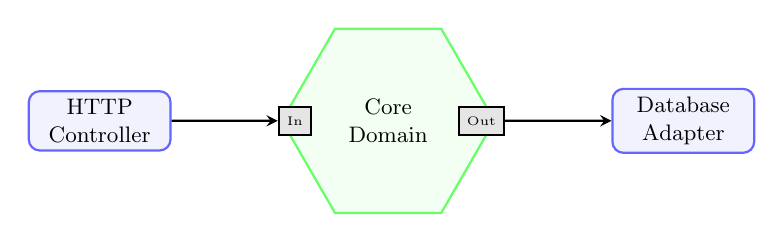
\begin{tikzpicture}[scale=0.9, transform shape,
    node distance=1.5cm,
    core/.style={draw, thick, regular polygon, regular polygon sides=6, minimum size=3cm, fill=green!5, draw=green!60, align=center, font=\small},
    port/.style={draw, thick, fill=gray!20, minimum size=0.4cm, font=\tiny},
    adapt/.style={draw, thick, rounded corners, fill=blue!5, draw=blue!60, minimum width=2cm, minimum height=0.8cm, align=center, font=\small},
    arrow/.style={draw, thick, ->, >=stealth}
]
    % Core
    \node[core] (core) {Core\\Domain};
    
    % Ports
    \node[port] (inport) at ([xshift=0.2cm]core.west) {In};
    \node[port] (outport) at ([xshift=-0.2cm]core.east) {Out};
    
    % Adapters
    \node[adapt, left=1.5cm of inport] (inadapt) {HTTP\\Controller};
    \node[adapt, right=1.5cm of outport] (outadapt) {Database\\Adapter};
    
    % Connections
    \draw[arrow] (inadapt) -- (inport);
    \draw[arrow] (outport) -- (outadapt);
\end{tikzpicture}
\caption{Hexagonal Architecture Dependency Flow}
\label{fig:hexflow}
\end{figure}

\section{Domain Interaction Map}
Figure~\ref{fig:domain_map} outlines how the core business domain layers communicate.

\begin{figure}[H]
\centering
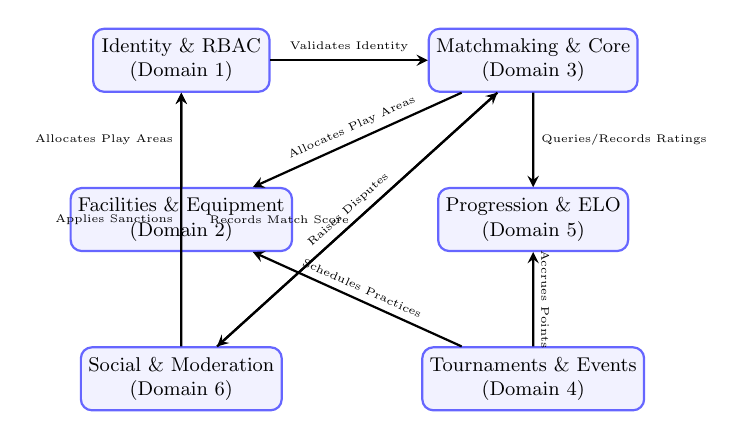
\begin{tikzpicture}[scale=0.8, transform shape,
    node distance=1.5cm and 2.5cm,
    dmn/.style={draw, thick, rounded corners, fill=blue!5, draw=blue!60, minimum width=2.8cm, minimum height=1cm, align=center, font=\small},
    arrow/.style={draw, thick, ->, >=stealth}
]
    % Nodes
    \node[dmn] (identity) {Identity \& RBAC\\(Domain 1)};
    \node[dmn, right=of identity] (matchmaking) {Matchmaking \& Core\\(Domain 3)};
    \node[dmn, below=of matchmaking] (progression) {Progression \& ELO\\(Domain 5)};
    \node[dmn, below=of identity] (facilities) {Facilities \& Equipment\\(Domain 2)};
    \node[dmn, below=of facilities] (social) {Social \& Moderation\\(Domain 6)};
    \node[dmn, below=of progression] (tournaments) {Tournaments \& Events\\(Domain 4)};
    
    % Connections with specific translated labels
    \draw[arrow] (identity) -- node[above, font=\tiny] {Validates Identity} (matchmaking);
    \draw[arrow] (matchmaking) -- node[right, font=\tiny] {Queries/Records Ratings} (progression);
    \draw[arrow] (facilities) -- node[left, font=\tiny] {Allocates Play Areas} (identity);
    \draw[arrow] (matchmaking) -- node[above, sloped, font=\tiny] {Allocates Play Areas} (facilities);
    
    \draw[arrow] (social) -- node[left, font=\tiny] {Applies Sanctions} (identity);
    \draw[arrow] (matchmaking) -- node[left, font=\tiny] {Records Match Score} (social);
    \draw[arrow] (social) -- node[above, sloped, font=\tiny] {Raises Disputes} (matchmaking);
    
    \draw[arrow] (tournaments) -- node[above, sloped, font=\tiny] {Accrues Points} (progression);
    \draw[arrow] (tournaments) -- node[above, sloped, font=\tiny] {Schedules Practices} (facilities);
    
\end{tikzpicture}
\caption{Domain Interaction Map}
\label{fig:domain_map}
\end{figure}

\section{Entity Relationship Diagram (ERD)}
Figure~\ref{fig:erd_layout} represents the primary entity relationship layout of the system.

\begin{figure}[H]
\centering
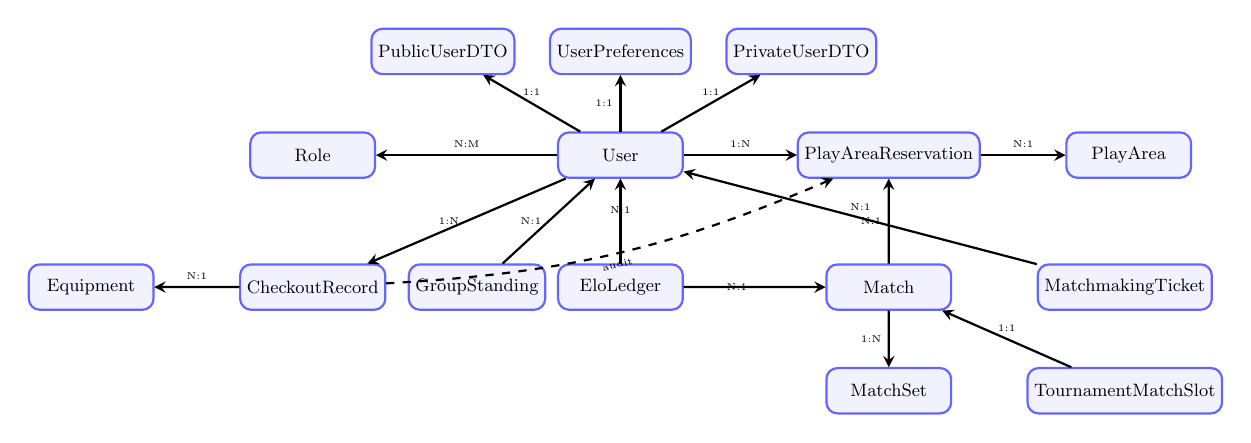
\begin{tikzpicture}[scale=0.72, transform shape,
    node distance=1cm and 1.5cm,
    ent/.style={draw, thick, rounded corners, fill=blue!5, draw=blue!60, minimum width=2.2cm, minimum height=0.8cm, align=center, font=\small},
    rel/.style={draw, thick, ->, >=stealth}
]
    \node[ent] (user) {User};
    \node[ent, above=of user] (pref) {UserPreferences};
    \node[ent, left=3.2cm of user] (role) {Role};
    \node[ent, left=0.6cm of pref] (pubdto) {PublicUserDTO};
    \node[ent, right=0.6cm of pref] (privdto) {PrivateUserDTO};
    
    % Facilities
    \node[ent, right=2cm of user] (res) {PlayAreaReservation};
    \node[ent, right=of res] (area) {PlayArea};
    \node[ent, below=1.5cm of role] (loan) {CheckoutRecord};
    \node[ent, left=of loan] (eq) {Equipment};
    
    % Core Matchmaking
    \node[ent, below=1.5cm of res] (match) {Match};
    \node[ent, right=of match] (ticket) {MatchmakingTicket};
    \node[ent, below=of match] (set) {MatchSet};
    \node[ent, below=1.5cm of user] (ledger) {EloLedger};
    \node[ent, left=0.2cm of ledger] (standing) {GroupStanding};
    \node[ent, below=of ticket] (slot) {TournamentMatchSlot};
    
    % Paths
    \draw[rel] (user) -- node[left, font=\tiny] {1:1} (pref);
    \draw[rel] (user) -- node[above, font=\tiny] {N:M} (role);
    \draw[rel] (user) -- node[above, font=\tiny] {1:1} (pubdto);
    \draw[rel] (user) -- node[above, font=\tiny] {1:1} (privdto);
    
    \draw[rel] (user) -- node[above, font=\tiny] {1:N} (res);
    \draw[rel] (res) -- node[above, font=\tiny] {N:1} (area);
    
    \draw[rel] (user) -- node[left, font=\tiny] {1:N} (loan);
    \draw[rel] (loan) -- node[above, font=\tiny] {N:1} (eq);
    
    \draw[rel] (ticket) -- node[above, font=\tiny] {N:1} (user);
    \draw[rel] (match) -- node[left, font=\tiny] {N:1} (res);
    \draw[rel] (match) -- node[left, font=\tiny] {1:N} (set);
    \draw[rel] (ledger) -- node[above, font=\tiny] {N:1} (user);
    \draw[rel] (ledger) -- node[left, font=\tiny] {N:1} (match);
    \draw[rel] (standing) -- node[left, font=\tiny] {N:1} (user);
    \draw[rel] (slot) -- node[above, font=\tiny] {1:1} (match);
    \draw[rel, dashed] (loan) to [bend right=10] node[below, sloped, font=\tiny] {audit} (res);
    
\end{tikzpicture}
\caption{Full Entity Relationship Diagram (ERD) Layout}
\label{fig:erd_layout}
\end{figure}

\section{Matchmaking Sequence}
Figure~\ref{fig:workflow_seq} displays the message flow during a successful player matchmaking request.

\begin{figure}[H]
\centering
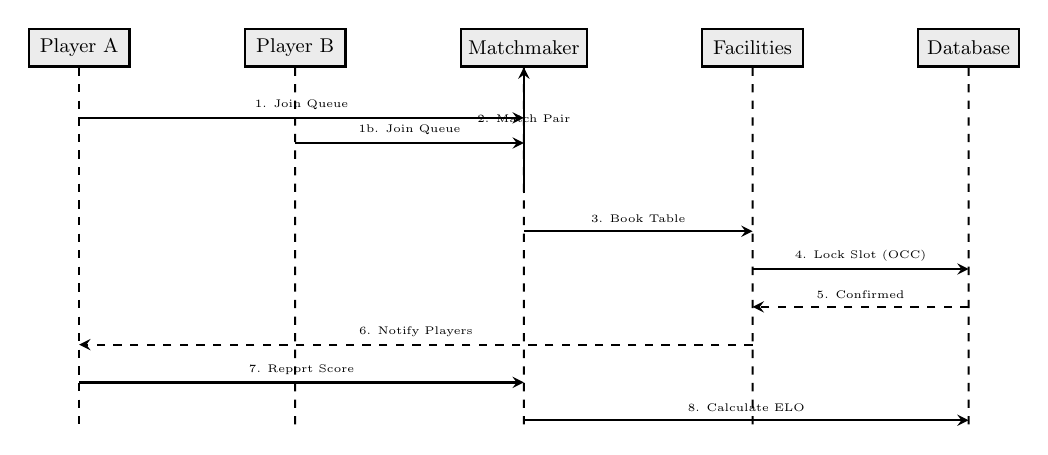
\begin{tikzpicture}[scale=0.8, transform shape,
    node distance=1cm and 1.8cm,
    lifeline/.style={draw, thick, dashed, minimum height=6.5cm},
    box/.style={draw, thick, fill=gray!15, minimum width=1.6cm, minimum height=0.6cm, align=center, font=\small},
    arrow/.style={draw, thick, ->, >=stealth}
]
    % Lifelines
    \node[box] (pA) {Player A};
    \node[box, right=of pA] (pB) {Player B};
    \node[box, right=of pB] (mm) {Matchmaker};
    \node[box, right=of mm] (fac) {Facilities};
    \node[box, right=of fac] (db) {Database};
    
    \draw[thick, dashed] (pA) -- ++(0,-6);
    \draw[thick, dashed] (pB) -- ++(0,-6);
    \draw[thick, dashed] (mm) -- ++(0,-6);
    \draw[thick, dashed] (fac) -- ++(0,-6);
    \draw[thick, dashed] (db) -- ++(0,-6);
    
    % Flow steps
    \draw[arrow] ([yshift=-0.8cm]pA.south) -- node[above, font=\tiny] {1. Join Queue} ([yshift=-0.8cm]mm.south);
    \draw[arrow] ([yshift=-1.2cm]pB.south) -- node[above, font=\tiny] {1b. Join Queue} ([yshift=-1.2cm]mm.south);
    \draw[arrow] ([yshift=-2.0cm]mm.south) -- node[above, font=\tiny] {2. Match Pair} (mm.south);
    \draw[arrow] ([yshift=-2.6cm]mm.south) -- node[above, font=\tiny] {3. Book Table} ([yshift=-2.6cm]fac.south);
    \draw[arrow] ([yshift=-3.2cm]fac.south) -- node[above, font=\tiny] {4. Lock Slot (OCC)} ([yshift=-3.2cm]db.south);
    \draw[arrow, dashed] ([yshift=-3.8cm]db.south) -- node[above, font=\tiny] {5. Confirmed} ([yshift=-3.8cm]fac.south);
    \draw[arrow, dashed] ([yshift=-4.4cm]fac.south) -- node[above, font=\tiny] {6. Notify Players} ([yshift=-4.4cm]pA.south);
    \draw[arrow] ([yshift=-5.0cm]pA.south) -- node[above, font=\tiny] {7. Report Score} ([yshift=-5.0cm]mm.south);
    \draw[arrow] ([yshift=-5.6cm]mm.south) -- node[above, font=\tiny] {8. Calculate ELO} ([yshift=-5.6cm]db.south);
    
\end{tikzpicture}
\caption{Matchmaking Flow and Facility Reservation Sequence}
\label{fig:workflow_seq}
\end{figure}

\section{Consolidated Backend Topology}
Figure~\ref{fig:consolidated_topo} outlines the physical instances and load balancing structure of scaled nodes.

\begin{figure}[H]
\centering
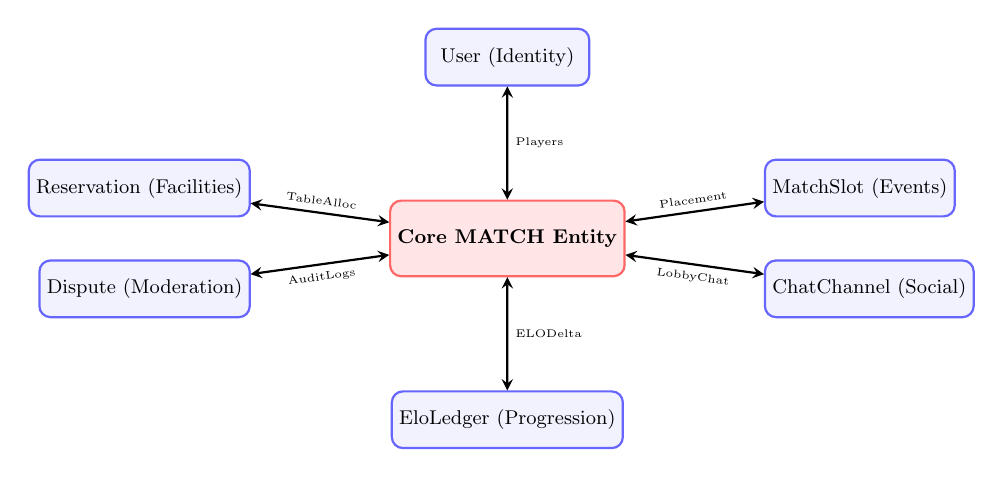
\begin{tikzpicture}[scale=0.8, transform shape,
    node distance=1.5cm and 2cm,
    central/.style={draw, thick, rounded corners, fill=red!10, draw=red!60, minimum width=3cm, minimum height=1.2cm, align=center, font=\bfseries\small},
    dmn/.style={draw, thick, rounded corners, fill=blue!5, draw=blue!60, minimum width=2.6cm, minimum height=0.9cm, align=center, font=\small},
    arrow/.style={draw, thick, <->, >=stealth}
]
    % Central Node
    \node[central] (match) {Core MATCH Entity};
    
    % Domain links around it
    \node[dmn, above=1.8cm of match] (identity) {User (Identity)};
    \node[dmn, below=1.8cm of match] (progression) {EloLedger (Progression)};
    \node[dmn, left=2.2cm of match, yshift=0.8cm] (facilities) {Reservation (Facilities)};
    \node[dmn, left=2.2cm of match, yshift=-0.8cm] (moderation) {Dispute (Moderation)};
    \node[dmn, right=2.2cm of match, yshift=0.8cm] (events) {MatchSlot (Events)};
    \node[dmn, right=2.2cm of match, yshift=-0.8cm] (social) {ChatChannel (Social)};
    
    % Path connections showing synthesis
    \draw[arrow] (match) -- node[right, font=\tiny] {Players} (identity);
    \draw[arrow] (match) -- node[right, font=\tiny] {ELODelta} (progression);
    \draw[arrow] (match) -- node[above, sloped, font=\tiny] {TableAlloc} (facilities);
    \draw[arrow] (match) -- node[below, sloped, font=\tiny] {AuditLogs} (moderation);
    \draw[arrow] (match) -- node[above, sloped, font=\tiny] {Placement} (events);
    \draw[arrow] (match) -- node[below, sloped, font=\tiny] {LobbyChat} (social);
    
\end{tikzpicture}
\caption{Consolidated Match-Centric Domain Linkage}
\label{fig:consolidated_topo}
\end{figure}

\section{Client Connectivity State Machine}
Figure~\ref{fig:statemachine} defines the client connection lifecycles, retries, and jitter policies, which are cross-referenced with the Zustand store and Capacitor mobile hooks.

\begin{figure}[H]
\centering
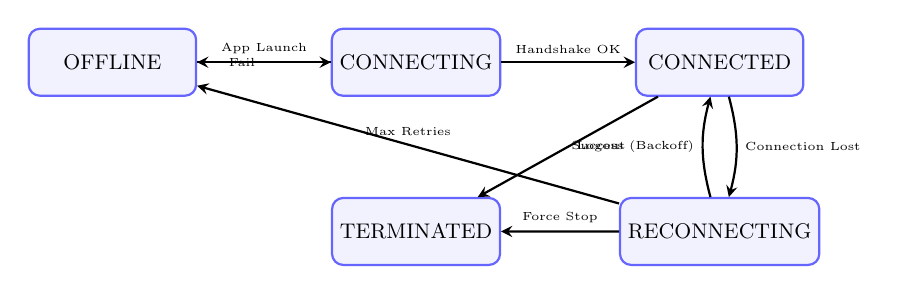
\begin{tikzpicture}[scale=0.85, transform shape,
    node distance=1.5cm and 2cm,
    state/.style={draw, thick, rounded corners, minimum width=2.5cm, minimum height=1cm, align=center, fill=blue!5, draw=blue!60, font=\small},
    arrow/.style={draw, thick, ->, >=stealth}
]
    \node[state] (offline) {OFFLINE};
    \node[state, right=of offline] (connecting) {CONNECTING};
    \node[state, right=of connecting] (connected) {CONNECTED};
    \node[state, below=of connected] (reconnecting) {RECONNECTING};
    \node[state, below=of connecting] (terminated) {TERMINATED};
    
    \draw[arrow] (offline) -- node[above, font=\tiny] {App Launch} (connecting);
    \draw[arrow] (connecting) -- node[above, font=\tiny] {Handshake OK} (connected);
    \draw[arrow] (connected) to [bend left=15] node[right, font=\tiny] {Connection Lost} (reconnecting);
    \draw[arrow] (reconnecting) to [bend left=15] node[left, font=\tiny] {Success (Backoff)} (connected);
    \draw[arrow] (reconnecting) -- node[above, font=\tiny] {Max Retries} (offline);
    \draw[arrow] (connected) -- node[right, font=\tiny] {Logout} (terminated);
    \draw[arrow] (connecting) -- node[left, font=\tiny] {Fail} (offline);
    \draw[arrow] (reconnecting) -- node[above, font=\tiny] {Force Stop} (terminated);
    
\end{tikzpicture}
\caption{Client Connectivity State Machine}
\label{fig:statemachine}
\end{figure}

\section{Concurrency Lock Handling Sequence}
Figure~\ref{fig:locking_seq} showcases optimistic concurrency control handling when reserving resources with capacity bounds. Under this flow, Thread A commits successfully, updating version from 0 to 1, while Thread B aborts with an \texttt{OptimisticLockException} and immediately triggers the matchmaking priority re-queue.

\begin{figure}[H]
\centering
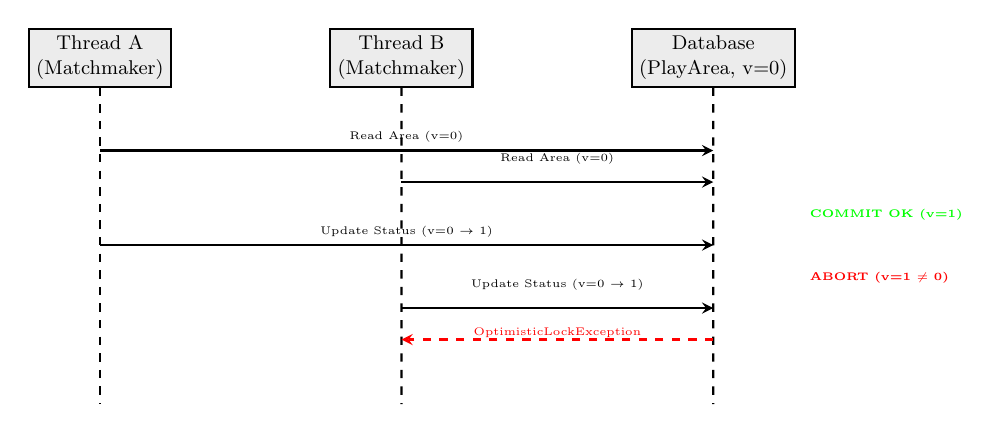
\begin{tikzpicture}[scale=0.8, transform shape,
    node distance=1cm and 2.5cm,
    lifeline/.style={draw, thick, dashed, minimum height=6cm},
    box/.style={draw, thick, fill=gray!15, minimum width=1.8cm, minimum height=0.6cm, align=center, font=\small},
    arrow/.style={draw, thick, ->, >=stealth}
]
    % Lifelines
    \node[box] (tA) {Thread A\\(Matchmaker)};
    \node[box, right=of tA] (tB) {Thread B\\(Matchmaker)};
    \node[box, right=of tB] (db) {Database\\(PlayArea, v=0)};
    
    \draw[thick, dashed] (tA) -- ++(0,-5.5);
    \draw[thick, dashed] (tB) -- ++(0,-5.5);
    \draw[thick, dashed] (db) -- ++(0,-5.5);
    
    % Flow
    \draw[arrow] ([yshift=-1cm]tA.south) -- node[above, font=\tiny] {Read Area (v=0)} ([yshift=-1cm]db.south);
    \draw[arrow] ([yshift=-1.5cm]tB.south) -- node[above, yshift=0.15cm, font=\tiny] {Read Area (v=0)} ([yshift=-1.5cm]db.south);
    
    \draw[arrow] ([yshift=-2.5cm]tA.south) -- node[above, font=\tiny] {Update Status (v=0 $\rightarrow$ 1)} ([yshift=-2.5cm]db.south);
    \node[right=0.1cm of db, yshift=-2.5cm, text=green, font=\tiny\bfseries] {COMMIT OK (v=1)};
    
    \draw[arrow] ([yshift=-3.5cm]tB.south) -- node[above, yshift=0.15cm, font=\tiny] {Update Status (v=0 $\rightarrow$ 1)} ([yshift=-3.5cm]db.south);
    \node[right=0.1cm of db, yshift=-3.5cm, text=red, font=\tiny\bfseries] {ABORT (v=1 $\neq$ 0)};
    \draw[arrow, dashed, red] ([yshift=-4cm]db.south) -- node[above, yshift=-0.1cm, text=red, font=\tiny] {OptimisticLockException} ([yshift=-4cm]tB.south);
    
\end{tikzpicture}
\caption{Optimistic Lock Conflict handling for tableCount = 1}
\label{fig:locking_seq}
\end{figure}


\end{document}
